%description: Basic Book in English
%% Based on a TeXnicCenter-Template by Gyorgy SZEIDL.
%%%%%%%%%%%%%%%%%%%%%%%%%%%%%%%%%%%%%%%%%%%%%%%%%%%%%%%%%%%%%

%----------------------------------------------------------
%
\documentclass[a4paper]{book}%
%
%----------------------------------------------------------
% This is a sample document for the standard LaTeX Book Class
% Class options
%       --  Body text point size:
%                        10pt (default), 11pt, 12pt
%       --  Paper size:  letterpaper (8.5x11 inch, default)
%                        a4paper, a5paper, b5paper,
%                        legalpaper, executivepaper
%       --  Orientation (portrait is the default):
%                        landscape
%       --  Printside:   oneside, twoside (default)
%       --  Quality:     final(default), draft
%       --  Title page:  titlepage, notitlepage
%       --  Columns:     onecolumn (default), twocolumn
%       --  Start chapter on left:
%                        openright(no, default), openany
%       --  Equation numbering (equation numbers on right is the default):
%                        leqno
%       --  Displayed equations (centered is the default):
%                        fleqn (flush left)
%       --  Open bibliography style (closed bibliography is the default):
%                        openbib
% For instance the command
%          \documentclass[a4paper,12pt,reqno]{book}
% ensures that the paper size is a4, fonts are typeset at the size 12p
% and the equation numbers are on the right side.
%
\usepackage{amsmath}%
\usepackage{amsfonts}%
\usepackage{amssymb}%
\usepackage{graphicx}
\usepackage{pdfpages}


\usepackage{ngerman}
\usepackage[latin1]{inputenc}
\usepackage[T1]{fontenc}
\usepackage{graphicx}
\usepackage{pdfpages} 
\usepackage{listings}
\usepackage{float}
\usepackage{verbatim}
%\usepackage{here}
\usepackage{booktabs}
\setlength{\parindent}{0pt}

%----------------------------------------------------------
\newtheorem{theorem}{Theorem}
\newtheorem{acknowledgement}[theorem]{Acknowledgement}
\newtheorem{algorithm}[theorem]{Algorithm}
\newtheorem{axiom}[theorem]{Axiom}
\newtheorem{case}[theorem]{Case}
\newtheorem{claim}[theorem]{Claim}
\newtheorem{conclusion}[theorem]{Conclusion}
\newtheorem{condition}[theorem]{Condition}
\newtheorem{conjecture}[theorem]{Conjecture}
\newtheorem{corollary}[theorem]{Corollary}
\newtheorem{criterion}[theorem]{Criterion}
\newtheorem{definition}[theorem]{Definition}
\newtheorem{example}[theorem]{Example}
\newtheorem{exercise}[theorem]{Exercise}
\newtheorem{lemma}[theorem]{Lemma}
\newtheorem{notation}[theorem]{Notation}
\newtheorem{problem}[theorem]{Problem}
\newtheorem{proposition}[theorem]{Proposition}
\newtheorem{remark}[theorem]{Remark}
\newtheorem{solution}[theorem]{Solution}
\newtheorem{summary}[theorem]{Summary}
\newenvironment{proof}[1][Proof]{\textbf{#1.} }{\ \rule{0.5em}{0.5em}}


\setcounter{tocdepth}{4}
%----------------------------------------------------------
\begin{document}

\frontmatter
\title{RTPbond - Strange things RTP}
\author{Alexander Vensmer, J\"urgen Schmidt, Martin Schwarz, Mike M\"uller \\ and Franz Streibl}
%\date{This whitepaper is licensed under the \\ GNU Free Documentation License Version 1.3 \\ \\ Stuttgart, 2009}
\maketitle
\tableofcontents

\chapter*{Preface}

This is the preface and it is created using a TeX field in a
paragraph by itself containing \verb|\chapter*{Preface}|. When the
document is loaded, this appears if it were a normal chapter, but
it is actually an unnumbered chapter. The \verb|markboth| TeX
field at the beginning of this paragraph sets the correct page
heading for the Preface portion of the document. The preface does
not appear in the table of contents.

\chapter{Introduction}

The introduction is entered using the usual chapter command. Since
the introduction chapter appears before the \verb|mainmatter| TeX
field, it is again an unnumbered chapter. The primary difference
between the preface and the introduction in this sample document
is that the introduction will appear in the table of contents and
the page headings for the introduction are automatically handled
without the need for the \verb|markboth| TeX field. You may use
either or both methods to create chapters at the beginning of your
document. You may also delete these preliminary chapters.

\mainmatter
\chapter{Protocol and Topology Considerations}




%\section{Netzwerk}
%\subsection{ISO Schichtenmodell}
\section{Network}
\subsection{ISO layer model}


%Als Basis fr viele heutige Kommunikationsprotokolle wird das OSI-Schichtenmodell verwendet. Sinn dieses Protokolls ist es ein komplettes Kommunikationsprotokoll in einzelne Schichten zu unterteilen. Diese Schichten kommunizieren jeweils nur mit ihren direkten Nachbarschichten, \ref{fig:OSI-Schichtenkommunikation} soll dies verdeutlichen. Dabei geht die Abstrahierung von der untersten Schicht, der Bitbertragungsschicht (engl.: physical Layer), bis zur siebten Schicht der Anwendungsschicht (engl.: Application-Layer).
%In der Bitbertragungsschicht werden die grundlegenden physikalischen Spezifikationen der bertragung wie zum Beispiel Strom-, Spannungswerte, Pinbelegung oder auch Abschlusswiderstnde festgelegt. Repeater, die in einem Netzwerk eingesetzt werden arbeiten immer auf dieser untersten Schicht.
%Im Gegensatz dazu wird in der Anwendungsschicht direkt mit den Netzwerkressourcen gearbeitet und Daten knnen direkt an den Empfnger gesendet werden ohne das Kenntnis ber Pinbelgung, Stromwerte oder andere physikalische Begebenheiten bentigt werden. Um dies  zu erreichen wird von der untersten Schicht bis zur Anwendungsschicht zwischen jeder Schicht abstrahiert, so kmmert sich die zweite Schicht, die sogenannte Sicherungsschicht (engl.: Data Link Layer) um die fehlerfreie Verbindung zwischen zwei benachbarten Netzwerkelementen. Schicht drei, welche Netzwerkschicht (engl.: Network-Layer) genannt wird, muss sich nicht mehr mit den Details der Datenbertragung befassen. Die Netzwerkschicht kann davon ausgehen, dass die Pakete sicher ankommen und befasst sich daher nur noch mit der Verwaltung der Pakete und dem Auffinden des effektivsten Weges fr ein Paket durch das Netzwerk (Routing). Alle Router in einem Netzwerk arbeiten daher auf dieser dritten Schicht.

Many modern protocols used for communication are based on the OSI layer model. This model divides a complete protocol into several seperate layers which only communicate with their directly adjacent layers, as shown in \ref{fig:OSI-Schichtenkommunikation}. We abstract from the bottom layer, the so called physical layer, upto the seventh layer, called application layer.\\
In the physical layer the basic specifications of the transmission are described, e.g. current, voltage, pin usage or termination impedances. Repeaters that are used in a network always operate in this lowest layer.\\
In contrast, in the application layer one can directly access network ressources and send data to the receiver without any knowledge of pin usage, voltage and other physical properties. To achieve this, we abstract from the bottom layer upto the application through several intermediate layer. Layer 2, the so called data link layer ensures errorless conections between to neighbours in the network. Layer 3, the network layer does not have to cope with the details of data transmission anymore. The network layer can rely on the fact, that all the packets arrive at the other side and so it can focus on routing. Therefore, all routers in the network operate in this network layer.


%\begin{figure}[H]
%	\centering
%	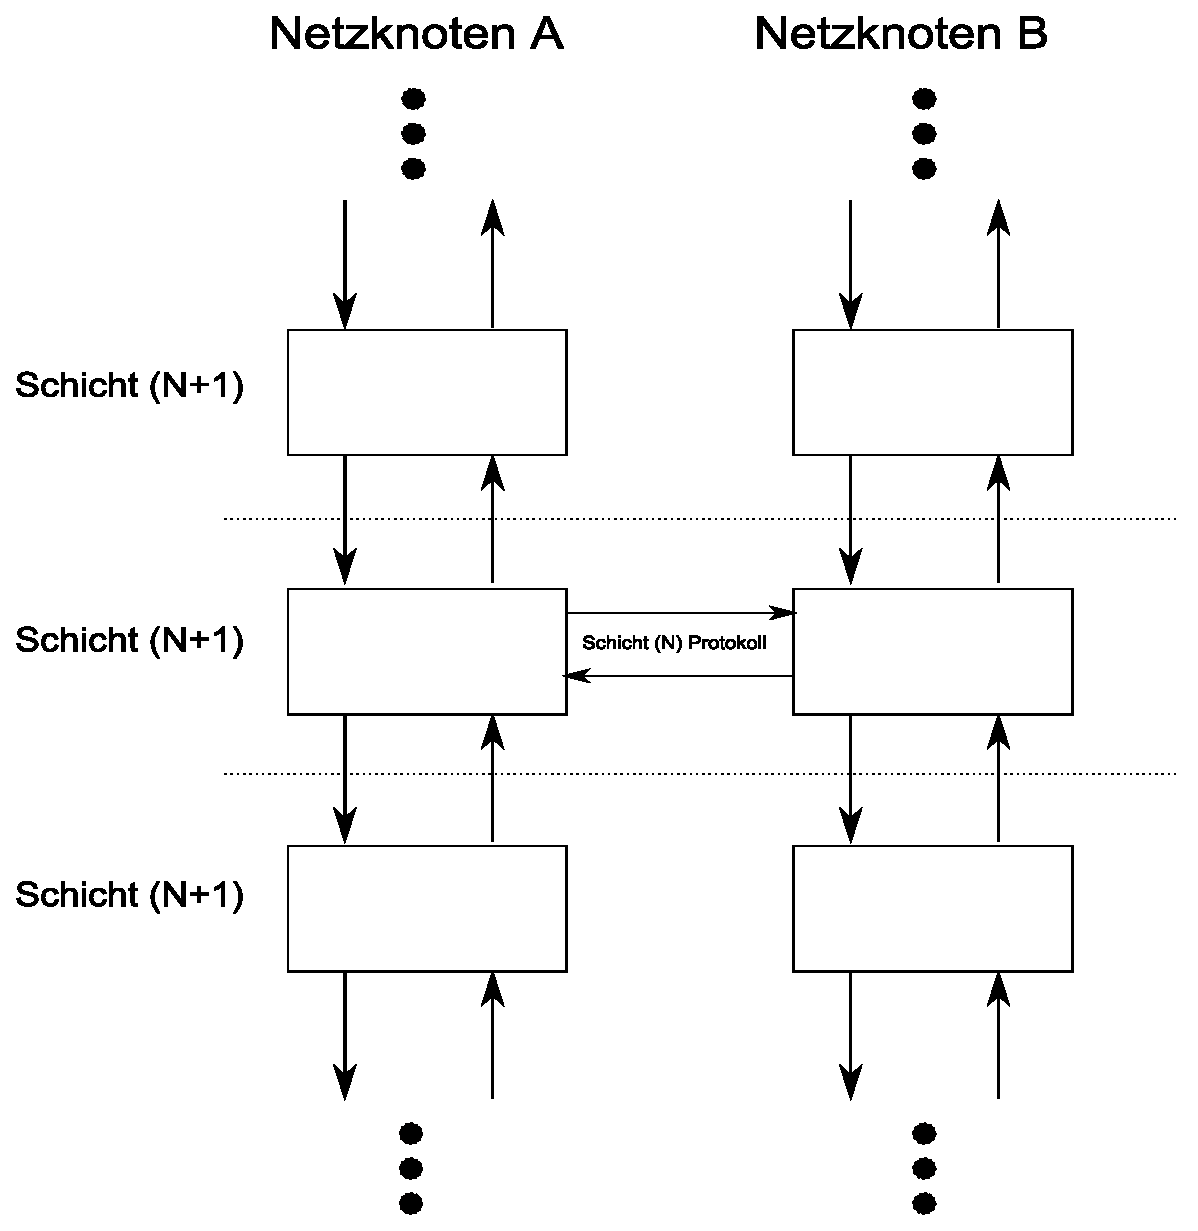
\includegraphics[width=1.0\textwidth]{figures/schichtkommunikation.eps}
%	\caption[Kommunikation zwischen OSI-Schichten]{Kommunikation zwischen OSI-Schichten}
%	\label{fig:OSI-Schichtenkommunikation}
%\end{figure}
\begin{figure}[H]
	\centering
	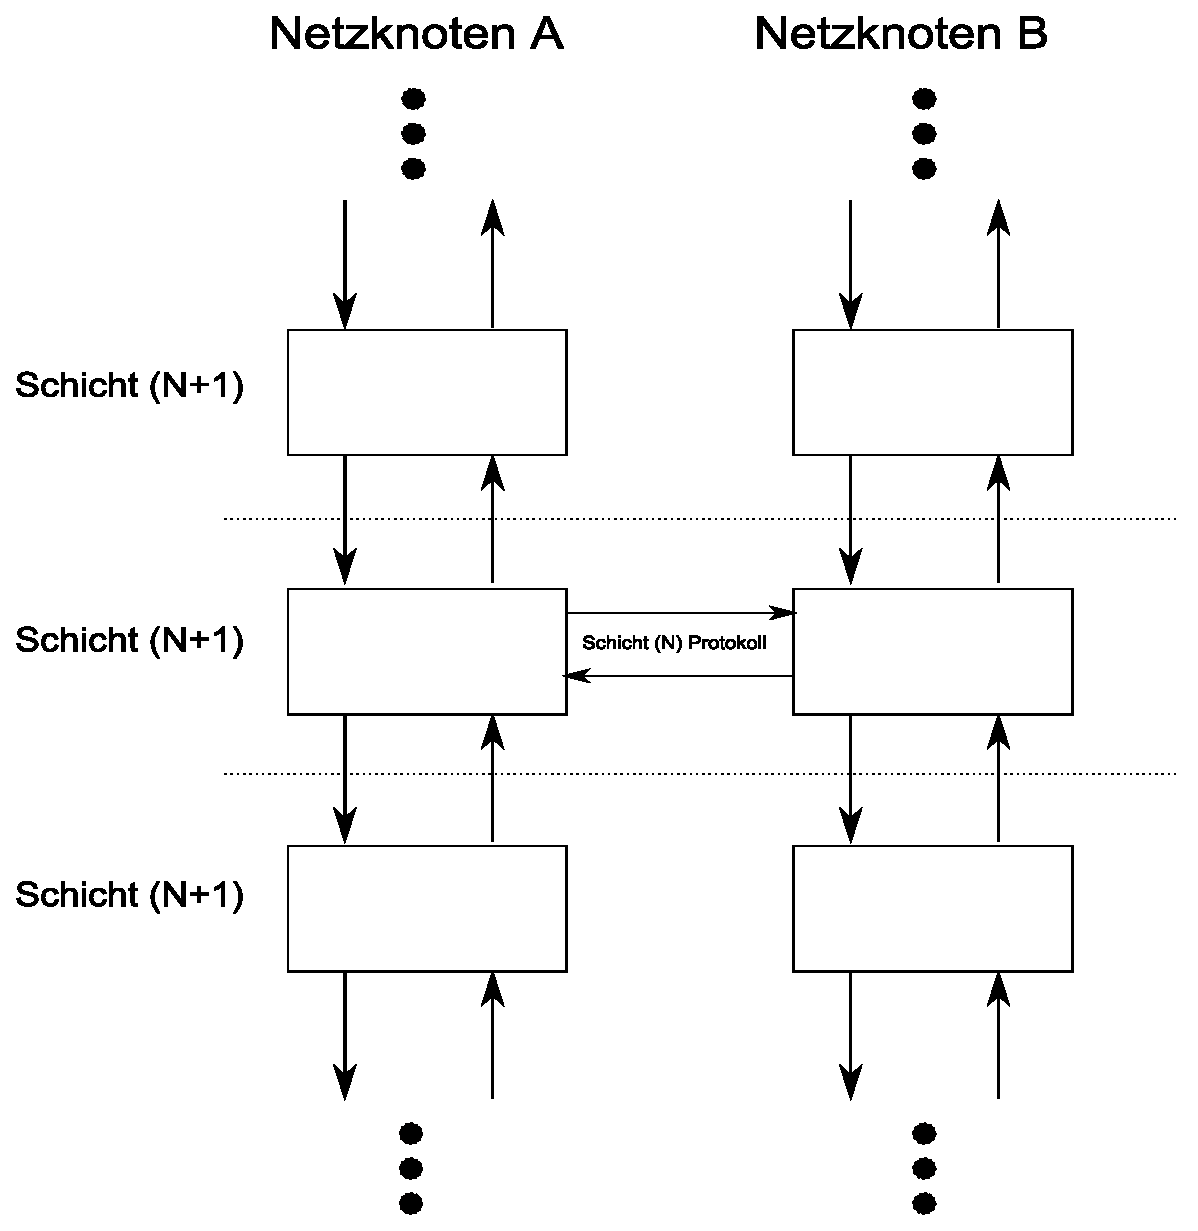
\includegraphics[width=1.0\textwidth]{figures/schichtkommunikation.eps}
	\caption[Communication between the OSI layers]{Kommunikation zwischen OSI-Schichten}
	\label{fig:OSI-Schichtenkommunikation}
\end{figure}


%\subsection{Die Schichten des OSI-Modells im berblick}
\subsection{Overview of the OSI layers}

\subsubsection{Layer 1: Physical Layer}
%Verbindungsschicht zur physikalischen Ebene. Verantwortung fr bertragung einzelner Bits.
Connection layer to the physical properties. Responsible for the transmission of single bits.

\subsubsection{Layer 2: Data Link Layer} 
%Die Sicherungsschicht sorgt fr eine zuverlssige und funktionierende Verbindung zwischen Endgert und bertragungsmedium. Zur Vermeidung von bertragungsfehlern und Datenverlust enthlt diese Schicht Funktionen zur Fehlererkennung, Fehlerbehebung und Datenflusskontrolle.
%Auf dieser Schicht findet auch die physikalische Adressierung von Datenpaketen statt.
The Data Link Layer establishes an errorless and reliable connection between endpoint and transmissionchannel. To avoid errors and data loss, this layer provides functions for error detection and error correction.\\
This layer also adresses the data packets physically.

\subsubsection{Layer 3: Network Layer}
%Die Vermittlungsschicht steuert die zeitliche und logische getrennte Kommunikation zwischen den Endgerten, unabhngig vom bertragungsmedium und -topologie. Auf dieser Schicht erfolgt erstmals die logische Adressierung der Endgerte. Die Adressierung ist eng mit dem Routing (Wegfindung vom Sender zum Empfnger) verbunden.
The Network Layer controls the communication between endpoints, independent from communication channels and topology. On this layer the endpoints are adressed logically. This adressation is strongly connected with the routing process (finding a way from sender to receiver).

\subsubsection{Layer 4: Transport Layer}
%Die Transportschicht ist das Bindeglied zwischen den transportorientierten und anwendungsorientierten Schichten. Hier werden die Datenpakete einer Anwendung zugeordnet.
The Transport Layer is the connection between the transportcentered and applicationcentered layers. In this layer, data packets are assigned to applications.

\subsubsection{Layer 5: Session Layer}
%Auf dieser Schicht wird der Verbindungsaufbau festgelegt und falls es bei der bertragung zu Fehlern kommt werden diese hier abgefangen und 
%ausgewertet.
%TODO: Hier weitermachen

\subsubsection{Schicht 6: Darstellungsschicht (Presentation Layer)}
Auf dieser Ebene werden Dateneingabe und -ausgabe berwacht und bertragungskonventionen festgelegt oder auch Bildschirmdarstellungen angepasst.

\subsubsection{Schicht 7: Anwendungsschicht (Application Layer)}
Die Anwendungsschicht stellt Funktionen fr die Anwendungen zur Verfgung. Auf dieser Schicht baut die Anwendung meist drauf auf und kann 
die Daten an die unteren Schichten weitergeben.

\newpage

\subsection{Realisierung des OSI-Modells}


Um die Realisierung des Netzwerkinterfaces zu vereinfachen wurden auch bei dem Messadapter die einzelnen Schichten des OSI-Modells realisert.
Die Anwendungs- und Prsentaionsschicht werden mit einem eigens hierfr entwickelten Protokoll dem CDP (Control Data Protokoll) sowie dem Real-Time Transport Protocol (RTP) umgesetzt. Die Sitzungsschicht und Transportschicht werden vom User Datagram Protocol (UDP) realisert. Schicht drei, die Netzwerkschicht, wird vom IP-Protokoll umgesetzt und die beiden letzten Schichten werden vom Ethernet spezifiziert.




\subsection{CDP}
Das CDP ist sehr klein und einfach gehalten. Es beinhaltet einmal die Kontrolle der Lnge der Nutzdaten, sowie einen Zeitstempel. Auch ist durch einen reservierten Speicherbereich die Mglichkeit der einfachen, abwrtskompatiblen Erweiterung mglich.

\subsection{RTP}
Real-Time Transport Protocol (RTP) wurde entwickelt, um Echtzeitdatenstrme ber ein Netzwerk zu transportieren. Es findet hufig Anwendung in der Telekommunikation und wird zum Beispiel von den in der IP-Technologie verwendeten Protokollen H.323 und SIP dazu verwendet, die Audio-/Videostrme eines Gesprches zu bertragen.
Es biete unter anderem die Mglichkeit festzuhalten, zu welchem Zeitpunkt das Paket gehrt oder auch durch einen Identifier mehrere Datenstrme \"parallel\" zu bertragen. Dies wird auch bei dem Messadapter genutzt um zwischen Datenstrmen und Konfigurationsbefehlen fr den ENC28J60 zu unterscheiden.


\subsection{UDP}

Das User Datagram Protocol, auch kurz UDP genannt, ist ein Netzwerkprotokoll das auf der Netzwerkschicht arbeitet. Es ist im Vergleich zu dem sehr bekannten Transmission Control Protocol (TCP) nicht verbindungsorientiert, daher ist UDP verbindungslos.
Bei einem verbindungsorientiertem Protokoll wird vor der eigentlichen Datenbertragung ein Drei-Wege-Handshake ausgefhrt. Auch wird festgehalten welche Pakete eines Datenrahmens bereits erfolgreich empfangen wurden und welche noch nicht. Dies geschieht ber ein Acknowledge-Pakete des Empfngers. Bei verbindungsorientierten Netzwerkprotokollen knnen also keine Daten verloren gehen, allerdings schafft diese Kontrolle darber einen relativ groen Overhead, was zur Verringerung der Nutzdatenbertragungsgeschwindigkeit fhrt. Dies war auch 1977 der Grund warum UDP berhaupt entwickelt wurde. Es wurde ein Protokoll bentigt mit dem Sprache sehr schnell transportiert werden konnte. Bei dem Versenden von Sprache und Video und allgemein aller Echtzeitdaten steht die Geschwindigkeit im Vordergrund, dazu kommt noch das ein verloren gegangenes Paket zu spterer Zeit nicht mehr fr die Verarbeitung verwendet werden kann da es fr den Zeitpunkt dann als ungltig betrachtet werden muss. Daher ist das in Hinsicht Vollstndigkeit etwas schlechtere Protokoll UDP, seinem verwandten TCP, bei Echtzeitdatenbertragung, vorzuziehen.


\subsection{IP}
Das Internet Protocol(IP) ist auf der (Internetschicht) zustndig fr den Transport von Daten ber mehrere Adressenbereiche(Subnetze) hinweg. Dabei nimmt das Internetprotocol beim versenden Daten vom TCP oder UDP entgegen und prft anhand der MTU (Maximum Transmission Unit) ob die Daten fragmentiert werden mssen, fr diese dann entstehenden Datagramme, oder das entstehende Datagramm bei geringer Datenmenge, wird ein Leitweg zum Ziel bestimmt. Datagramme werden von Gateways von Netz zu Netz weitergeleitet, bis sie ihr Ziel erreicht haben oder der TTL-Zhler der an jeder Netzwerkstation decrementiert wird den Wert Null erreicht, was das sofortige fallen lassen des Paketes zur Folge hat. Das IP stellt einen Adressierungsmechanismus zur Verfgung, welcher die Wegwahl zwischen Netzwerken ermglicht. Dieser bentigt die im Header abgelegten Informationen der Quell- und Zieladresse. Mit diesen 

\subsection{Ethernet}

Ethernet arbeitet auf den zwei untersten Schichten OSI-Referenzmodells und deckt damit die Bitbertragungsschicht sowie die Sicherungsschicht ab. Ethernet ist also die Verbindung zur physikalischen Ebene und den oberen immer abstrakter werdenden Schichten.
Der erste Standard des Ethernets wurde erstmals auf der 10 Base 5-Implementierung des IEEE festgeschrieben. Die maximale Datengeschwindigkeit betrug damals bei diesem Basisbandbertragungsverfahren 10MBit/s. Auch wenn das heutzutage sich am meisten im Einsatz befindende Ethernet 100Base-T (IEEE 802.3 Clause 24) eine bertragung von 100MBit/s aufweist existiert bereits das so genannte Gigabit Ethernet mit dem eine bertragungsgeschwindigkeit von 10 000Mbit/s erreicht werden kann. Das 10Gigabit-Ethernet ist in der 1000BaseX-Implementierung und ihren Untergruppen definiert.
Whrend in der ersten Generation noch mit Kabeln die einen halben Zoll dick waren, so genannte Thick Ethernet  Kabel, gearbeitet wurde, werden beim 100Base-T Kabel flexible 6mm dicke twisted-pair Kabel, so genannte Thin Ethernet Kabel, verwendet. Das Gigabit Ethernet sendet seine Daten vornehmlich ber Glasfaserkabel. 
Das Ethernet-Protokoll sieht nicht vor das die Binrsignale direkt ber das betreffende Kabel geschickt wird, da bei dieser Methode der Empfnger nicht entscheiden kann, wann ein Bit anfngt oder endet. Deshalb wird hier die so genannte Manchester-Codierung eingesetzt. Bei der Manchester-Codierung wird jedes Bit in zwei gleichlange Intervalle unterteilt. Falls das erste Intervall auf dem high-Pegel liegt und das zweite auf dem low-Pegel interpretiert der Empfnger das Bit als eine logische 1. Eine logische 0 wird bei umgekehrter Reihenfolge detektiert. Durch diese Codierung ist sichergestellt, dass whrend der Dauer, die zur bertragung eines Datenbits bentigt wird, auf jeden Fall eine Pegelnderung stattfindet. Ein weiterer Vorteil auer der sehr einfachen Synchronisierungsmglichkeit des Empfngers ist, dass sich auf dem Kabel kein gleichfrmiges Signal bildet. Ein Nachteil ist allerdings, dass die Bandbreite doppelt so gro sein muss wie bei reiner Bitcodierung da die Pulsbreite nur noch halb so gro ist.
Um diesen Nachteil zu mildern wurde beim bergang vom 10BaseT zum 100BaseT die Manchester Codierung erweitert zur 4B/5B-Umwandlung. Bei dieser Umwandlung werden aus den Daten jeweils 4Bit herausgenommen und dann so in 5Bit umgewandelt, dass in jedem sich ergebenen 5Bit Block maximal 2Nullen enthalten sind, daraus ergibt sich dann Umwandlungstabelle \ref{tab:umwandlung} die natrlich Sender und Empfnger bekannt ist.
 

\begin{table}
\caption{4Bit/5Bit Umwandlung Manchseter-Codierung}
\label{tab:umwandlung}
\centering
\begin{tabular}{llll}\toprule
(4-Bit-Block) & (5-Bit-Block) \\ \midrule
0000 &	11110 \\
0001 &	01001 \\
0010 &	10100 \\
0011 &	10101 \\
0100 &	01010 \\
0101 &	01011 \\
0110 &	01110 \\
0111 &	01111 \\
1000 &	10010 \\
1001 &	10011 \\
1010 &	10110 \\
1011 &	10111 \\
1100 &	11010 \\
1101 &	11011 \\
1110 &	11100 \\
1111 &	11101 \\ \bottomrule
\end{tabular}
\vspace{5 mm}
\end{table}



Falls also die Bitfolge: \newline
1010 0001 1011 0010 \newline
gesendet werden soll so wrde auf dem Bus die dekodierte bitfolge:\newline
10110 01001 10111 10100\newline
anliegen. Wie auch Abbildung \ref{fig:manu} zeigt.

\begin{figure}[H]
	\centering
	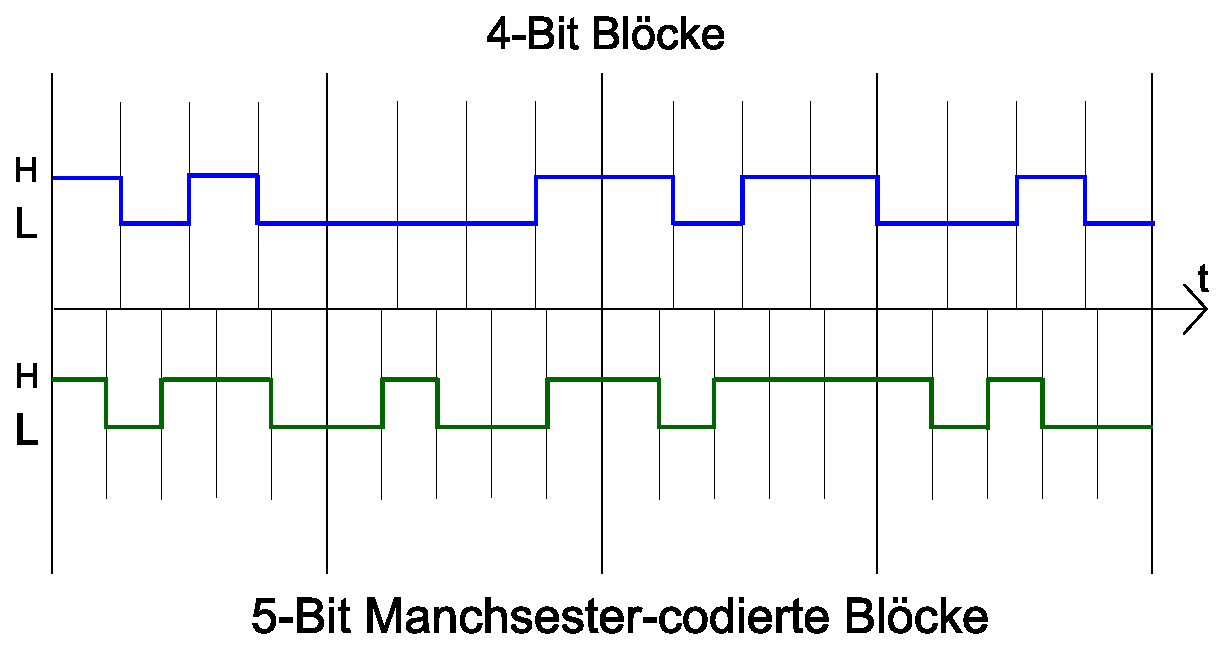
\includegraphics[width=1.0\textwidth]{figures/manchester.eps}
	\caption[Beispiel Manchester-Codierung]{Beispiel Manchester-Codierung}
	\label{fig:manu}
\end{figure}

Der Zugriff auf das Ethernet-Kabel wird vom Media Access Control (MAC) geregelt. MAC arbeitet auf der Schicht 2 des OSI-Referenzmodells und stellt somit einen wichtigen Teil vom Ethernet da. Der im MAC-Standard enthaltene CSMA/CD-Mechanismus behandelt alle Netzwerkteilnehmer gleich. Dies ist dadurch realisiert, dass Alle Ethernet-Stationen haben jederzeit und immer uneingeschrnkten Zugriff auf das Netz. Der CSMA/CD (Carrier Sense Multiple Access/Collision Detection)-Mechanismus ein Teil von MAC steuert den Zugriff auf das bertragungsmedium. Vor dem Senden von Daten wird getestet, ob das Medium zum senden frei (Carrier Sense) oder besetzt ist. Ist das Medium frei wird das Senden gestartet. Fr den Fall das eine weitere Ethernet-Station zur selben Zeit angefangen hat zu Senden, stellen die beide Netzteilnehmer fest und stoppen beide ihren Sendevorgang zudem wird noch ein jam-Signal auf das Kabel gelegt um sicherzugehen das alle Netzteilnehmer die Kollision ebenfalls entdecken. Nach einer zuflligen Zeitspanne versuchen beide Stationen nochmals zu senden.



\chapter{Linux Reference Application}
\section{\texttt{rtpbondd} Binary}
\subsection{Overview}

The \emph{rtpbondd} binary is a small daemon-like tool for Linux that permits users to transfer messages in our RTP/CDP packet format through the network. \emph{rtpbondd} reads the data to send from FIFOs and writes received data to other FIFOs from which they can be read and processed by the user or by other tools. The rtpbondd tool runs in the background and generates the required additional headers 

\subsection{Installation}

The \emph{rtpbondd} sourcecode is accompanied by the following Makefile which does all the work needed to generate a binary.

%\lstset{language=make}
%\lstset{caption=The Makefile}
%\lstset{captionpos=b}
%\begin{lstlisting}
\begin{verbatim}
# Makefile for rtpbondd.c
EXEC_RTPBONDD = rtpbondd
EXEC_RTPBONDD_BF = rtpbondd_bf
OBJS_RTPBONDD = rtpbondd.o
OBJS_RTPBONDD_BF = rtpbondd_bf.o
SRC_RTPBONDD = rtpbondd.c

#The configuration for the Linuxhost
LDFLAGS = -lpthread -o $@ -lm
INCLDIR = /usr/include

#The configuration for the DNP
CC_BF = /home/mike/opt/uClinux/bfin-uclinux/bin/bfin-uclinux-gcc
CFLAGS_BF = -Wl,-elf2flt
INCLDIR_BF = /home/mike/opt/uClinux/bfin-uclinux/bfin-uclinux/runtime/usr/include/
LIBDIR_BF = /home/mike/opt/uClinux/bfin-linux-uclibc/bfin-linux-uclibc/runtime/lib/
LDFLAGS_BF = -pthread -o $@ -lm -L$(LIBDIR_BF)
		
all: $(EXEC_RTPBONDD) 


$(EXEC_RTPBONDD): $(OBJS_RTPBONDD)
	$(CC) -I$(INCLDIR) $(LDFLAGS) $(OBJS_RTPBONDD) -lm -lc

$(OBJS_RTPBONDD):
	$(CC) -c -I$(INCLDIR) $(SRC_RTPBONDD)
	
dnp: $(EXEC_RTPBONDD_BF)

$(EXEC_RTPBONDD_BF): $(OBJS_RTPBONDD_BF)
	$(CC_BF) -I$(INCLDIR_BF) $(LDFLAGS_BF) $(CFLAGS_BF) $(OBJS_RTPBONDD_BF) -lm

$(OBJS_RTPBONDD_BF):
	$(CC_BF) -c -o $@ -I$(INCLDIR_BF) $(CFLAGS_BF) $(SRC_RTPBONDD)

clean:
	-rm -f $(EXEC_RTPBONDD) $(EXEC_RTPBONDD_BF) *.elf *.gdb *.o
\end{verbatim}

To compile the binary for a normal Linux PC you can use the standard target and just type:
\begin{verbatim}
$ make
\end{verbatim}

The Makefile also contains a buildtarget for the DNP/5370 board which can be called by:
\begin{verbatim}
$ make dnp
\end{verbatim}
%\end{lstlisting}

\subsection{Usage}
\subsubsection{Starting the program}

There are two possibilities to start the program. To just start the program and configure one device directly just use the following call:

\begin{verbatim}
$ rtpbondd deviceName destIp4Addr destPort listenPort (0 for any) baudRate[bytes/s] TMax[ms]
\end{verbatim}

There is also the possibility to configure some devices in a configfile, which will all be started by rtpbondd then. To do this, just append the name of the configfile to the programcall:

\begin{verbatim}
$ rtpbondd configfile
\end{verbatim}

\subsubsection{Sample configfile}

The structure of the configfile can be easily seen in the following example. The identation is just for better readabiliy and does not have to be used!


\begin{verbatim}
#this is a comment. it begins with # and has to be on its own line
deviceName              "FIFO1"
path                "/home/user/"
destIp4Addr         "129.69.176.127"
destPort            "1234"
listenPort          "43211"
baudRate[bytes/s]   "1000"
TMax[ms]            "1000"
payloadType         "37"

deviceName              "FIFO2"
path                "."
destIp4Addr         "129.69.176.129"
destPort            "34567"
listenPort          "56789"
baudRate[bytes/s]   "1500"
TMax[ms]            "2000"
payloadType         "77"
\end{verbatim}


\subsubsection{Sending/receiving data}

The program creates two FIFOs in the current working directory for every configured device: deviceName.payloadType.in und deviceName.payloadType.out
Received data can be read from deviceName.payloadType.in, e.g. with cat:

\begin{verbatim}
$ cat deviceName.payloadType.in
\end{verbatim}

Data can be sent by writing it into deviceName.payloadType.out, e.g. with echo:

\begin{verbatim}
$ echo "Hello World" > deviceName.payloadType.out"
\end{verbatim}

Received data can be read from deviceName.payloadType.in by other programs as well. And other programs can of course send data by writing into deviceName.payloadType.out.

\subsubsection{Getting the status}

The deviceconfiguration and connectionstats of a running rtpbondd process can be retrieved by entering

\begin{verbatim}
$ rtpbondd status
\end{verbatim}

The output looks similar to this:

\begin{verbatim}
Configfile loaded: rtpbondd.conf                         
2 device(s) running:                                    
FIFO1:                                                  
path: /home/user/                               
destIp4Addr: 129.69.176.127     destPort: 1234  
listenPort: 43211                               
baudRate: 1000  TMax: 1000                      
payloadType: 37                                 
Packets sent: 11 (0 data/11 alive)      Packets received: 0 (0 data/0 alive)    status: inactive
Avg payload sent: 0.00 byte      Avg payload received: 0.00 byte                                
Packets lost: 0                                                                                 
FIFO2:                                                                                                  
path: .                                                                                         
destIp4Addr: 129.69.176.129     destPort: 34567                                                 
listenPort: 56789                                                                               
baudRate: 1500  TMax: 2000                                                                      
payloadType: 77                                                                                 
Packets sent: 5 (0 data/5 alive)        Packets received: 0 (0 data/0 alive)    status: inactive
Avg payload sent: 0.00 byte      Avg payload received: 0.00 byte                                
Packets lost: 0             
\end{verbatim}

\subsubsection{Restarting a device}

A running device can be restarted by editing the appropriate configfile and calling:

\begin{verbatim}
$ rtpbondd restart deviceName
\end{verbatim}

The deviceName must not be changed of course!


\subsubsection{Troubleshooting}

If the following error occurs while starting the program

\begin{verbatim}
rtpbondd: error: bind(socketRecv) failed. ERRNO: 98
\end{verbatim}

then there is another rtpbondd process running on the system, using the same port. You have to end that one first, for example with killall:

\begin{verbatim}
$ killall rtpbondd
\end{verbatim}

%$ - highlighting help

\section{\texttt{rtpconf} Script}
\subsection{Overview}

The \emph{rtpconf} script is a command line tool to ease the usage of the introduced \emph{rtpbond}-setup. It is written completely in bash to allow best flexibility and portability in usage and expansion of features.

On software side, an end-user of a \emph{rtpbond}-setup will meet in most cases all his requirements in configuration and maintenance with \emph{rtpconf}.

\subsection{Features}

\begin{itemize}
\item Generating an overview of properties of all devices in setup
\item Changing properties (i.e. IP-address, port number, baudrate etc.)
\item Changing properties of remote devices through network connection
\item 'Easy to use' configuration-routine to customize the behavior of remote devices
\item Flexible instruction set to transmit possible future commands to remote devices
\item Error preventing user guiding
\end{itemize}

\subsection{Usage}
Under your bash terminal environment you can start \emph{rtpconf}.
\subsubsection{Starting with \emph{help}}
\begin{verbatim}
user@machine:~/rtpbond/rtpconf$ ./rtpconf
rtpconf v0.9.9 (2009/11/25)
> help
rtpconf v0.9.9 (2009/11/25)
Usage: ./rtpconf [command] [command-parameter/device]
If no command is committed, rtpconf will start in 'interactive mode'. All following commands can be used either in interactive mode or as a single command
* help        print this
* quit        quits the interactive mode (alias: exit)
* status      prints status output - if remote status available even this
* version     print current version of this script

Remote commands:
* open        opens a device for easy use
* close       close current opened device
* send        transmit text to device. first open a device or use syntax 'send FIFONAME TEXT'
* configure   starts a configuration routine to set up a remote device
* restart     restarts remote device (aliases: reset, reboot) ACHTUNG: BISHER NUR RESTART VON TTY_NET-THREAD
* dump        dump configuration for rtpbondd (based on internal device states)
* configtype  print/set payload-type for configuration channels
> quit
user@machine:~/rtpbond/rtpconf$
\end{verbatim}

\subsubsection{Status output}
Example with 4 devices configured in rtpbondd (called FIFO1, FIFO2, FIFO3, FIFO4). FIFO1 \& FIFO2 and FIFO3 \& FIFO4 are representing two physical remote devices. Each device consists of a configuration channel and a data transmisson channel (note: Payload Type '37' versus '77').

Global Status print:

\begin{verbatim}
rtpconf v0.9.9 (2009/11/25)
> stat
FIFO1:                                                  
	path: .                               
	destIp4Addr: 192.168.22.23     destPort: 9000  
	listenPort: 9000                               
	baudRate: 1000  TMax: 1000                      
	payloadType: 37                                 
	Packets sent: 11 (0 data/11 alive)      Packets received: 0 (0 data/0 alive)    status: inactive
	Avg payload sent: 0.00 byte      Avg payload received: 0.00 byte                                
	Packets lost: 0                                                                                 

	Availability check: Positive

	Remote Status:
	  IP: 192.168.22.23
	  Netmask: 255.255.255.0
	  Gateway: 192.168.22.1
	  Mac-Address: 00:00:00:00:00:01
	  Data_Dest_IP: 192.168.22.100
	  Data_Dest_Port: 9000
	  Config_Dest_IP: 192.168.22.100
	  Config_Dest_Port: 9000
	  Baudrate: 9600
FIFO2:                                                                                                  
	path: .                                                                                         
	destIp4Addr: 192.168.22.129     destPort: 34567                                                 
	listenPort: 56789                                                                               
	baudRate: 1500  TMax: 2000                                                                      
	payloadType: 77                                                                                 
	Packets sent: 5 (0 data/5 alive)        Packets received: 0 (0 data/0 alive)    status: inactive
	Avg payload sent: 0.00 byte      Avg payload received: 0.00 byte                                
	Packets lost: 0
FIFO3:                                                  
	path: .                               
	destIp4Addr: 192.168.22.42     destPort: 9001  
	listenPort: 9001                               
	baudRate: 1000  TMax: 1000                      
	payloadType: 37                                 
	Packets sent: 11 (0 data/11 alive)      Packets received: 0 (0 data/0 alive)    status: inactive
	Avg payload sent: 0.00 byte      Avg payload received: 0.00 byte                                
	Packets lost: 0                                                                                 

	Availability check: Positive

	Remote Status:
	  IP: 192.168.22.42
	  Netmask: 255.255.255.0
	  Gateway: 192.168.22.1
	  Mac-Address: 00:00:00:00:00:02
	  Data_Dest_IP: 192.168.22.100
	  Data_Dest_Port: 9001
	  Config_Dest_IP: 192.168.22.100
	  Config_Dest_Port: 9001
	  Baudrate: 115200
FIFO4:                                                                                                  
	path: .                                                                                         
	destIp4Addr: 192.168.22.131     destPort: 34567                                                 
	listenPort: 56789                                                                               
	baudRate: 1500  TMax: 2000                                                                      
	payloadType: 77                                                                                 
	Packets sent: 5 (0 data/5 alive)        Packets received: 0 (0 data/0 alive)    status: inactive
	Avg payload sent: 0.00 byte      Avg payload received: 0.00 byte                                
	Packets lost: 0
> 
\end{verbatim}

By selecting (\emph{opening}) a particular device it is much more clear and handy:
\begin{verbatim}
> open FIFO1
Selecting remote device 'FIFO1' ...
FIFO1> stat
Status of 'FIFO1'
FIFO1:                                                  
	path: .                               
	destIp4Addr: 192.168.22.23     destPort: 9000  
	listenPort: 9000                               
	baudRate: 1000  TMax: 1000                      
	payloadType: 37                                 
	Packets sent: 11 (0 data/11 alive)      Packets received: 0 (0 data/0 alive)    status: inactive
	Avg payload sent: 0.00 byte      Avg payload received: 0.00 byte                                
	Packets lost: 0                                                                                 

	Availability check: Positive

	Remote Status:
	  IP: 192.168.22.23
	  Netmask: 255.255.255.0
	  Gateway: 192.168.22.1
	  Mac-Address: 00:00:00:00:00:01
	  Data_Dest_IP: 192.168.22.100
	  Data_Dest_Port: 9000
	  Config_Dest_IP: 192.168.22.100
	  Config_Dest_Port: 9000
	  Baudrate: 9600
FIFO1>
\end{verbatim}

\section{Example}

\chapter{Microcontroller Reference Implementation}

\section{Hardware}
\section{Software}

\subsection{Sende- und Empfangsprozess der seriellen Brcke}

\subsubsection{COM-Schnittstelle RS-232}

Die RS-232 Schnittstelle allgemein bekannt auch als COM-Schnittstelle wurde bereits in den frhen 1960ern von einem US-amerikanischen Standardisierungskomitee (heute EIA - Electronic Industries Alliance) eingefhrt. Die RS232 gehrt zur Kategorie seriellen Datenverbindungen und ist sehr flexibel und einfach einsetzbar. Dies ist der Grund dafr dass diese Schnittstelle auch heute noch in der Industrie sehr hufig verwendet wird. Auch in der Messtechnik ist diese Schnittstelle noch sehr gebruchlich und kann auch bei High-End Gerten noch hufig angetroffen werden. Die Verbindung kann hierbei je nach Anforderung speziell auf jedes Gert eingestellt werden, man kann hier zum Beispiel die Anzahl der Datenbits zwischen eins und neun einstellen oder auch die Anzahl der Stoppbits festlegen. Die Stoppbits kennzeichnen jeweils das Ende eines Datenframes. Um eine mgliche Inkonsistenz der Daten bei bertragungsfehlern zu verringern gibt es zustzlich noch ein so genanntes Parittsbit. Dieses Parittsbit gibt an ob das Ergebnis einer XOR-Verknpfung der Datenbits gerade oder ungerade ist. Grundstzlich lsst sich mit der RS232 Schnittstelle ein synchroner aber auch ein asynchroner Datenaustausch zwischen den UARTs realisieren.
Ein UART ist ein elektronisches Bauelement, welches zur Realisierung von digitalen seriellen Schnittstellen dient. Eine UART-Schnittstelle dient zum Senden und Empfangen von Daten ber eine Datenleitung und bildet den Standard der seriellen Schnittstellen an PCs und Mikrocontrollern. 
Auch kann ber zustzliche Steuerleitungen Leitungen die Verbindung kontrolliert werden.
Es gibt unter anderem RTS (Request to Send) eine logische Null an diesem Ausgang signalisiert der Gegenstelle, dass sie Daten senden kann sowie das Signal CTS (Clear to Send) welches angibt das Daten empfangen werden knnen. Bei der Schnittstelle des Messadapter welche fr das Debugging verwendet wird werden diese beiden stndig auf logisch 0 gesetzt, daher nicht verwendet, es kann also gesendet werden auch wenn die Empfangstelle nicht bereit ist. Dafr dass die Schnittstelle nur zum Debugging verwendet werden soll reicht das allerdings vollkommen aus. Auf das Thema Debugging wird in einem spteren Kapitel nochmals genauer eingegangen.
Die Schnittstelle wird in unserem Fall mit einer Baud-Rate von 115,2KByte betrieben.



\subsubsection{ttyS0(RS232) to Ethernet}

Die Hauptaufgabe des Messadapters ist es Messungen anzuregen, daher Pakete vom Netzwerk entgegen zunehmen und dem Messgert zu schicken und daruafhin die gewonnen Messergebnisse wieder einem bestimmten Ethernet fhigem Gert zurck zusenden. Es soll hier nun nher auf die Datenrichtung vom Messgert zum Netzwerk eingegangen werden.
Um dies zu realisieren wird, falls Daten RS232 Schnittstelle ankommen, ein Interrupt ausgelst der die ankommenden Daten in einen davor vorgesehenen 150Byte  (kann per Compilerschalter COM0\_MAX\_RX\_BUF eingestellt werden)  groen Buffer geschrieben. Ist der Buffer voll soll dieser an den Netzwerkteilnehmer, der im EEPROM gespeichert ist, gesendet werden. Um das Echtzeitverhalten des Messadapters zu verbessern kann allerdings auch eine obere Schranke eingestellt werden ab welcher der Buffer schon frher gesendet werden, hierzu mehr in Kapitel \ref{chapter:konfig}.
Um einen stetigen Datenfluss von Ethernet-Paketen zu erreichen  sendet der Messadapter nicht nur ein Ethernet-Paket wenn der 150Byte groe Buffer voll ist, bzw. die angesprochene Schranke erreicht wird, sondern kann bei geringem Datenaufkommen, durch einen Timer gesteuert, schon frher  senden. Das wird auch im Programmablaufplan \ref{fig:aufbauPaket} gezeigt, man sieht, dass entweder ein abgelaufener Timer oder ein voller Buffer zu einem Aufruf der Funktion com0RotateRecvBuffer() fhrt.
Die Funktion com0RotateRcvBuffer() schreibt den Buffer, der bei keinem Datenaufkommen durchaus auch 0Bytes lang sein kann, als Element in die Ausgangs-FiFo-Queue (out-Fifo des Data Devices). Erst wenn in dieser FiFo-Queue ein Element bereit liegt wird der Messadapter senden.
Wie im Programmablaufplan \ref{fig:onmain} zu sehen ist, wird die Funktion OnSerial() stndig aufgerufen, die Funktion bergibt ein Element, bestehend aus dem Buffer der die angekommenen Daten der RS232-Schnittstelle enthlt, der Ausgangs-FiFo-Queue an die Funktion OnSerialData(). Die Funktion OnSerialData() ruft wiederum die Funktion rtpSendCDPData() auf.

\begin{figure}[H]
	\centering
	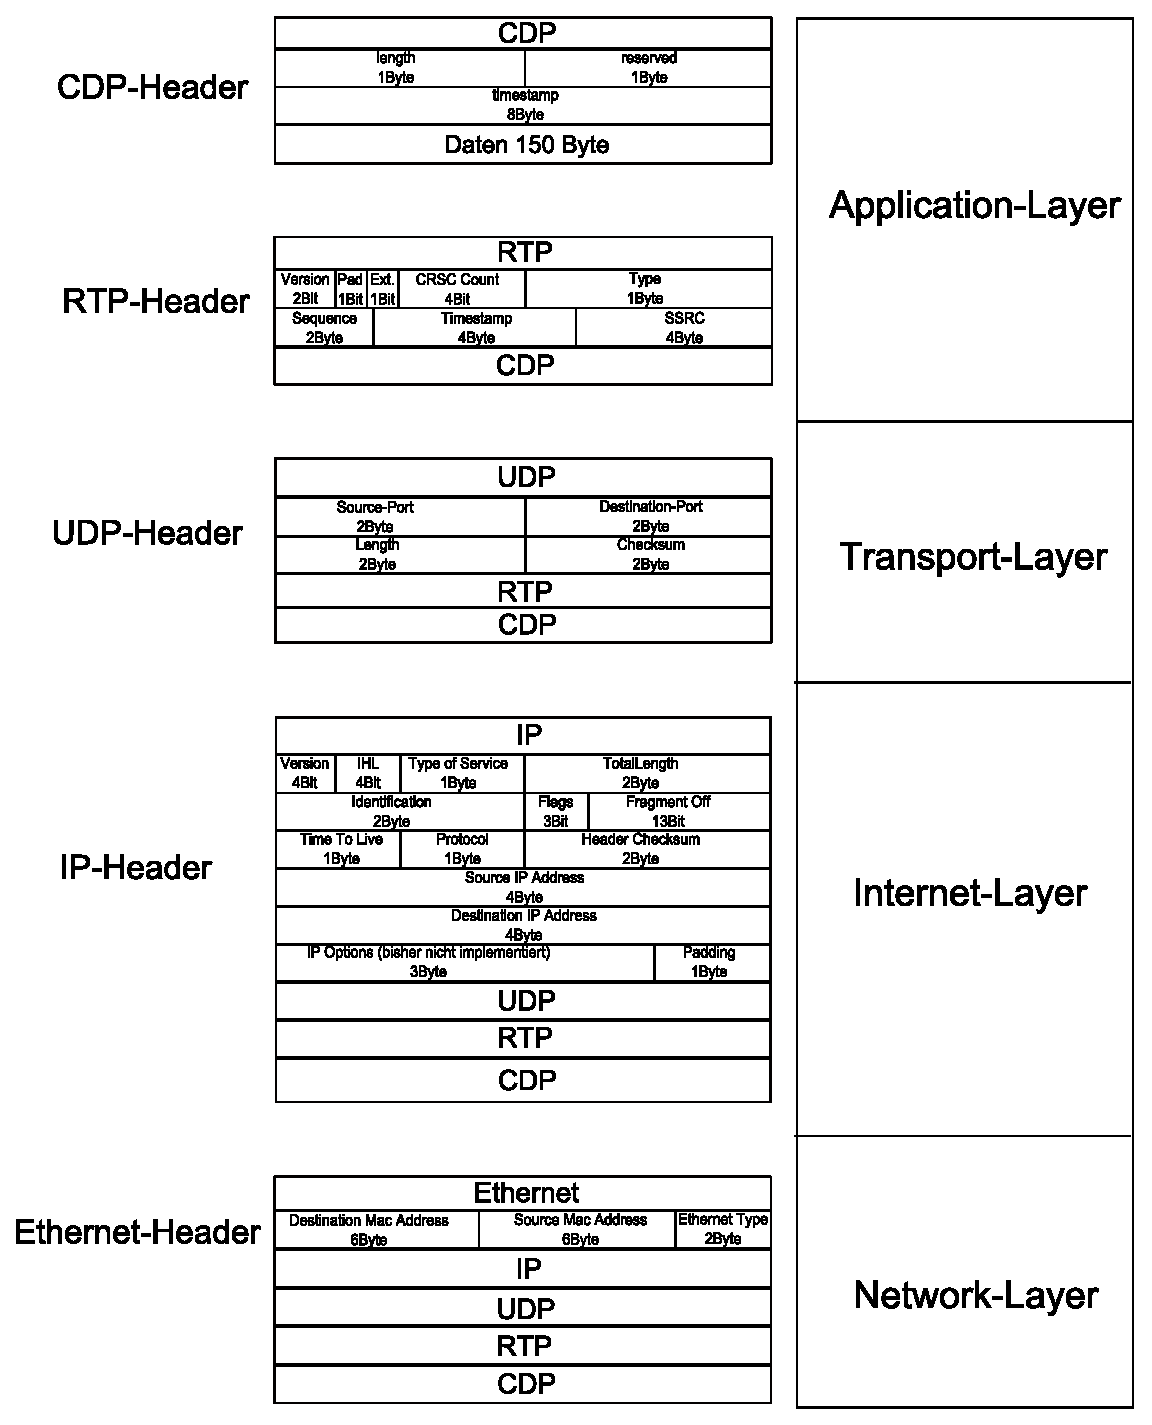
\includegraphics[width=1.0\textwidth]{figures/schrittweiseraufbaueinespaketes.eps}
	\caption[Aufbau eines kompletten CDP-Paketes]{Aufbau eines kompletten CDP-Paketes}
	\label{fig:aufbauPaket}
\end{figure}

\begin{figure}[H]
	\centering
	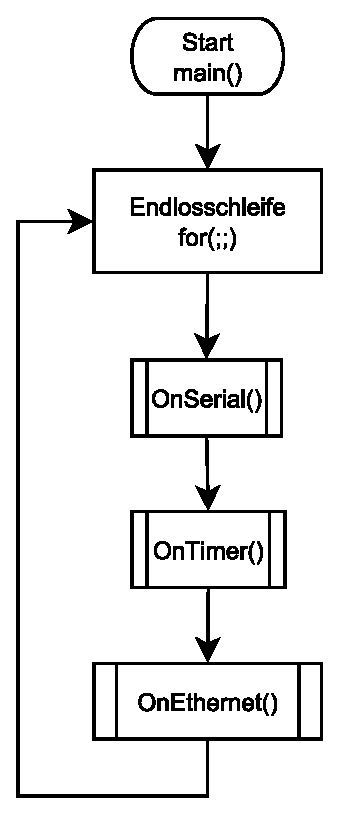
\includegraphics[width=0.2\textwidth]{figures/onmain.eps}
	\caption[Main-Funktion]{Main-Funktion}
	\label{fig:onmain}
\end{figure}

\begin{figure}[H]
	\centering
	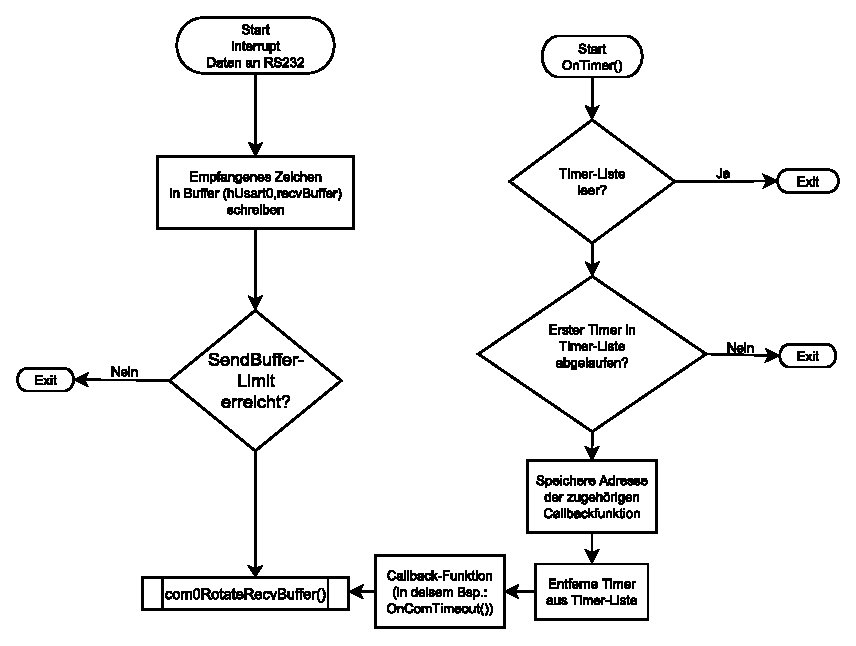
\includegraphics[width=0.8\textwidth]{figures/ontimer.eps}
	\caption[onTimer()]{onTimer()}
	\label{fig:ontimer}
\end{figure}


\begin{figure}[H]
	\centering
	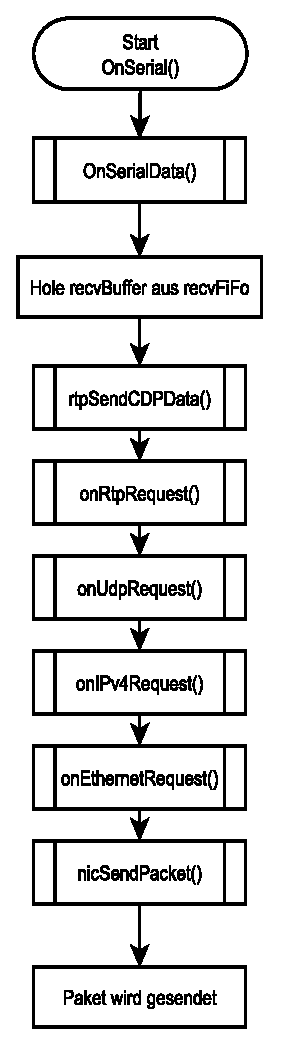
\includegraphics[width=0.2\textwidth]{figures/onserial.eps}
	\caption[onSerial()]{onSerial()}
	\label{fig:aonserial}
\end{figure}

\begin{figure}[H]
	\centering
	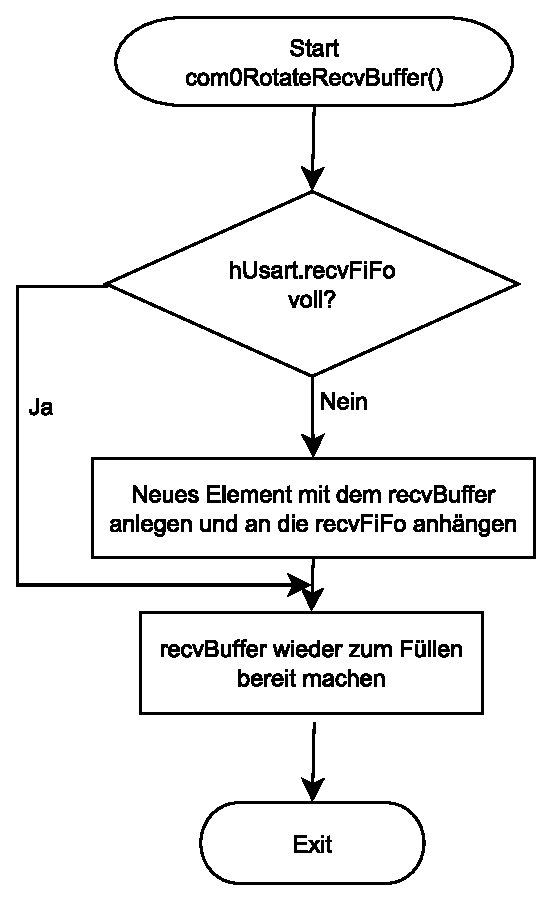
\includegraphics[width=0.3\textwidth]{figures/rotaterecvbuffer.eps}
	\caption[Rotate Reciver Buffer]{Rotate Reciver Buffer}
	\label{fig:rotaterecvbuffer}
\end{figure}

An dieser Stelle beginnt nun der inkrementelle Aufbau des Ethernet-Paketes, und damit auch die Realisierung der in Kapitel 1 betrachteten Schichten.
Dazu wird zuallererst eine allgemeine Paketstruktur mit einem Zeiger auf den Speicherbereich des spteren Headers  und einen Zeiger auf den Speicherbereich des Payloads angelegt.
Der Zeiger auf den Payload-Speicherbereich dieses innersten Pakets wird zu NULL gesetzt, um eine geschickte Abbruchbedingung fr eine Schleife beim eigentlichen Senden zu erhalten. In den Speicherbereich des Headers wird nun der CDP-Header sowie die Daten des zu sendenden Buffers geschrieben. Der CDP-Header besteht aus den drei in Kapitel 1 bereits erwhnten Speicherbereichen: Zum einen die Lnge der Daten und zum anderen ein  Feld fr die relative Systemzeit des Senders sowie ein Reserved-Byte das spter eventuell als Sub-Type Erkennung verwendet werden kann. Benutzt wird von diesen drei Feldern bisher allerdings nur das Lngen-Feld die anderen werden konstant zu 0 gesetzt. Das erhaltene Paket wird daraufhin der Funktion onRtpRequest() bergeben. Die Funktion onRtpRequest() legt wiederum eine wie oben beschriebene Paketstruktur an, setzt den Zeiger des Payloads aber diesmal auf das bereits angelegte Paket. Der Header wird nun mit den Daten eines RTP-Headers gefllt. Wie auch Abb. \ref{fig:speicherabbild} entnommen werden kann enthlt der RTP-Header einige wichtige Information bezglich Echtzeitdatenbertragung. Vom Messadapter verwendet wird das Versionsfeld in das konstant die 80 eingetragen wird, das Typenfeld welches angibt ob es sich um weitergeleitete Daten oder ein Steuerungsbefehl handelt hierbei steht die hexadezimalen Zahlen 4D fr Daten und die 25 fr Steuerungsbefehle, ein Feld fr einen Zeitstempel in dem die aktuell gelaufene Systemzeit in der Einheit 976,56 Mikrosekunden steht und ein Feld Sequenz das mit dem Wert eines einfachen Paketcounter befllt wird. 
Dieses erhaltene RTP-Paket wird daraufhin der Funktion onUdpRequest() bergeben die, die Daten eines UDP-Headers hinzufgen. Dieser Header enthlt den Quellport des Messadapters sowie den Zielport des Netzwerkgertes das die Ethernet-Pakete empfangen soll. Auerdem ist noch ein Feld fr eine Checksumme enthalten welches allerdings nicht benutzt wird sowie ein Lngen-Feld das die Lnge des bisher erstellten Paketes bergeben bekommt. Daraufhin wird dem Paket in der Funktion onIPv4Request()ein IP-Header angefgt. Die vom Messadapter benutzten Felder des IP-Header sind  einmal das Versionsfeld in dem die Version des benutzten IP-Headers gespeichert wird, das Type of Service Feld welches heutzutage kaum benutzt und auch vom Messadapter nicht in Benutzung genommen wird und zu 0 gesetzt, ein Lngen-Feld das die Lnge des bisher erstellten Paketes bergeben bekommt, das  Identifications-Feld das eine Seriennummer darstellt um zuerkennen welche Fragemente zu welchen IP-Paketen gehren und von einem Paketzhler gefllt wird, das Feld zur Bestimmung der Fragmentierung wird derart beschrieben das..,das Time To Live Feld wird mit der 128 gefllt und gibt die Anzahl der maximal zu passierenden Netzwerknoten an, das Protokoll-Feld wird mit der hexadezimalen 11 gefllt was angibt das es sich um ein UDP-Paket im Datenfeld des IP-Paketes handelt und zuletzt wird noch eine Prfsumme angehngt um die Konsistenz der Daten zu gewhrleisten. Aus dem neu entstandenem IP-Paket wird durch Anfgen eines Ethernet-Headers ein Ethernet-Paket gemacht. In dem angefgten Header steht zum einen die Mac-Adresse des Messadapters die aus dem EEPROM ausgelesen wird und zum anderen die Mac-Adresse des Netzwerkgertes, welche ber das Address Resolution Protocol in Erfahrung gebracht werden kann. Auerdem wird in dem Typen-Feld noch vermerkt das in dem Payloadbereich des Ethernet-Paketes sich ein IPv4 Paket befindet.
Die sich im Speicher dann ergebene Struktur ist in Abb. \ref{fig:speicherabbild} dargestellt.
Dieses Paket wird jetzt wieder Schrittweise dem Sendepuffer des ENC28J60 bergeben. Um das zu realisieren weist  Paketzeiger auf den Header des Ethernet-Paketes und bergibt diesen. Daraufhin wird der Zeiger auf den Payloadbereich umgesetzt was wiederum der Anfang des nchsten Headers (IP-Header) darstellt. Dieses umsetzen des Zeigers und senden wird solange gemacht bis der umgesetzte Zeiger auf NULL weist(Abbruchbedingung). Wenn dies passiert wurde das komplette Paket gesendet.




\begin{figure}[H]
	\centering
	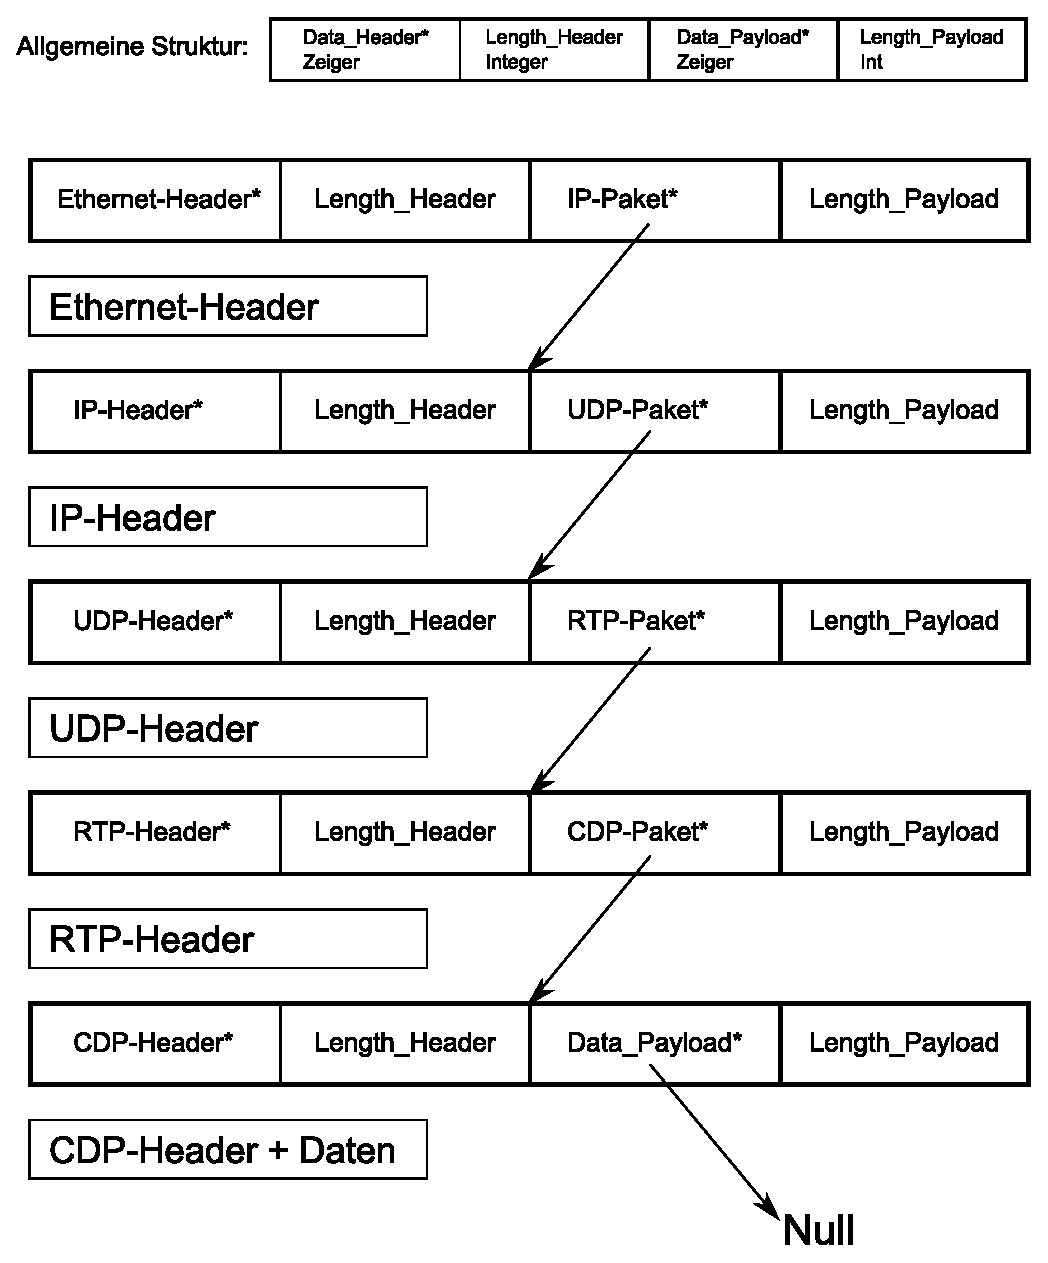
\includegraphics[width=1.0\textwidth]{figures/speicherabbild.eps}
	\caption[Aufbau eines CDP-Paketes im Speicher]{Aufbau eines CDP-Paketes im Speicher}
	\label{fig:speicherabbild}
\end{figure}



\subsubsection{Ethernet to ttyS0(RS232)}
Um ein Messgert zu steuern mssen Daten am Netzwerkinterface entgegen genommen und an die RS232 Schnittstelle weitergegeben werden knnen. Dieser Ablauf ist in Abb. \ref{fig:ethernettors232 part1} dargestellt. Zuallererst wird am ENC28J60 abgefragt werden ob angekommene Pakete bereitliegen. Falls ein Ethernet-Paket bereit liegt wird die Lnge des Paketes abgespeichert, zustzliche auch vorliegende Informationen wie zum Beispiel ob ein CRC Error vorlag oder der Opcode nicht erkannt wurde werden allerdings nicht ausgewertet. Nun wird angefangen Header fr Header des Paketes aus dem Empfangs-Buffer des ENC28J60 auszulesen. Angefangen wird dieser Prozess in der Funktion OnEthernetResponse(), welche den Ethernet-Header ausliest. Darauhin wird zunchst geprft ob die Datenlnge des eingelesenen Headers die richtige Lnge hat. Trifft dies zu, wird als nchstes mithilfe des Ethernet-Type Feldes ausgewertet ob ein ARP-Paket oder ein IP-Paket vorliegt. Im Falle eines ARP-Paketes wird mithilfe von Diesem der ARP-Cache aktualisiert. Falls ein  IP-Paket vorliegt wird der dazugehrige IP-Header ausgelesen und mithilfe des Destination IP Address Feldes geprft ob der Messadapter berhaupt der richtige Empfnger ist. Falls dies nicht der Fall ist wird das Paket sofort fallengelassen. Bei bereinstimmung der Adresse des Adapters aus dem EEPROM mit der Zieladresse aus dem IP-Header wird die Adresse des sendenden Netzwerkelementes in den ARP-Cache geschrieben. Beim darauf folgenden Test stellt sich heraus ob das Paket ein UDP-Paket ist. Ist das Paket ein UDP-Paket wird der UDP-Header eingelesen. Mithilfe von diesem Header kann festgestellt werden ob eine TFTP-Verbindung aufgenommen werden soll oder ob ein RTP-Paket mit Daten angekommen ist. Im Falle eines RTP-Paketes wird der RTP-Header ausgelesen. Nun kann anhand des RTP-Typen-Feldes festgestellt werden ob das Paket zum Schreiben beziehungsweise Lesen von Konfigurationseinstellungen gesendet wurde. Ist das Paket kein Konfigurationspaket sondern fr die RS232-Schnittstelle bestimmt werden die angekommenen Daten erst der Funktion onRtpData(), danach serialSendBytes() und schlielich der Funktion com0SendBytes() bergeben. Zum Senden der Daten wird zunchst festgestellt ob die FiFo zum senden leer oder gefllt ist. Bei einer nicht leeren FiFo-Queue wird der Buffer in dieser abgelegt. War die FiFo-Queue leer wird das senden der Daten direkt angeregt.



\begin{figure}[H]
	\centering
	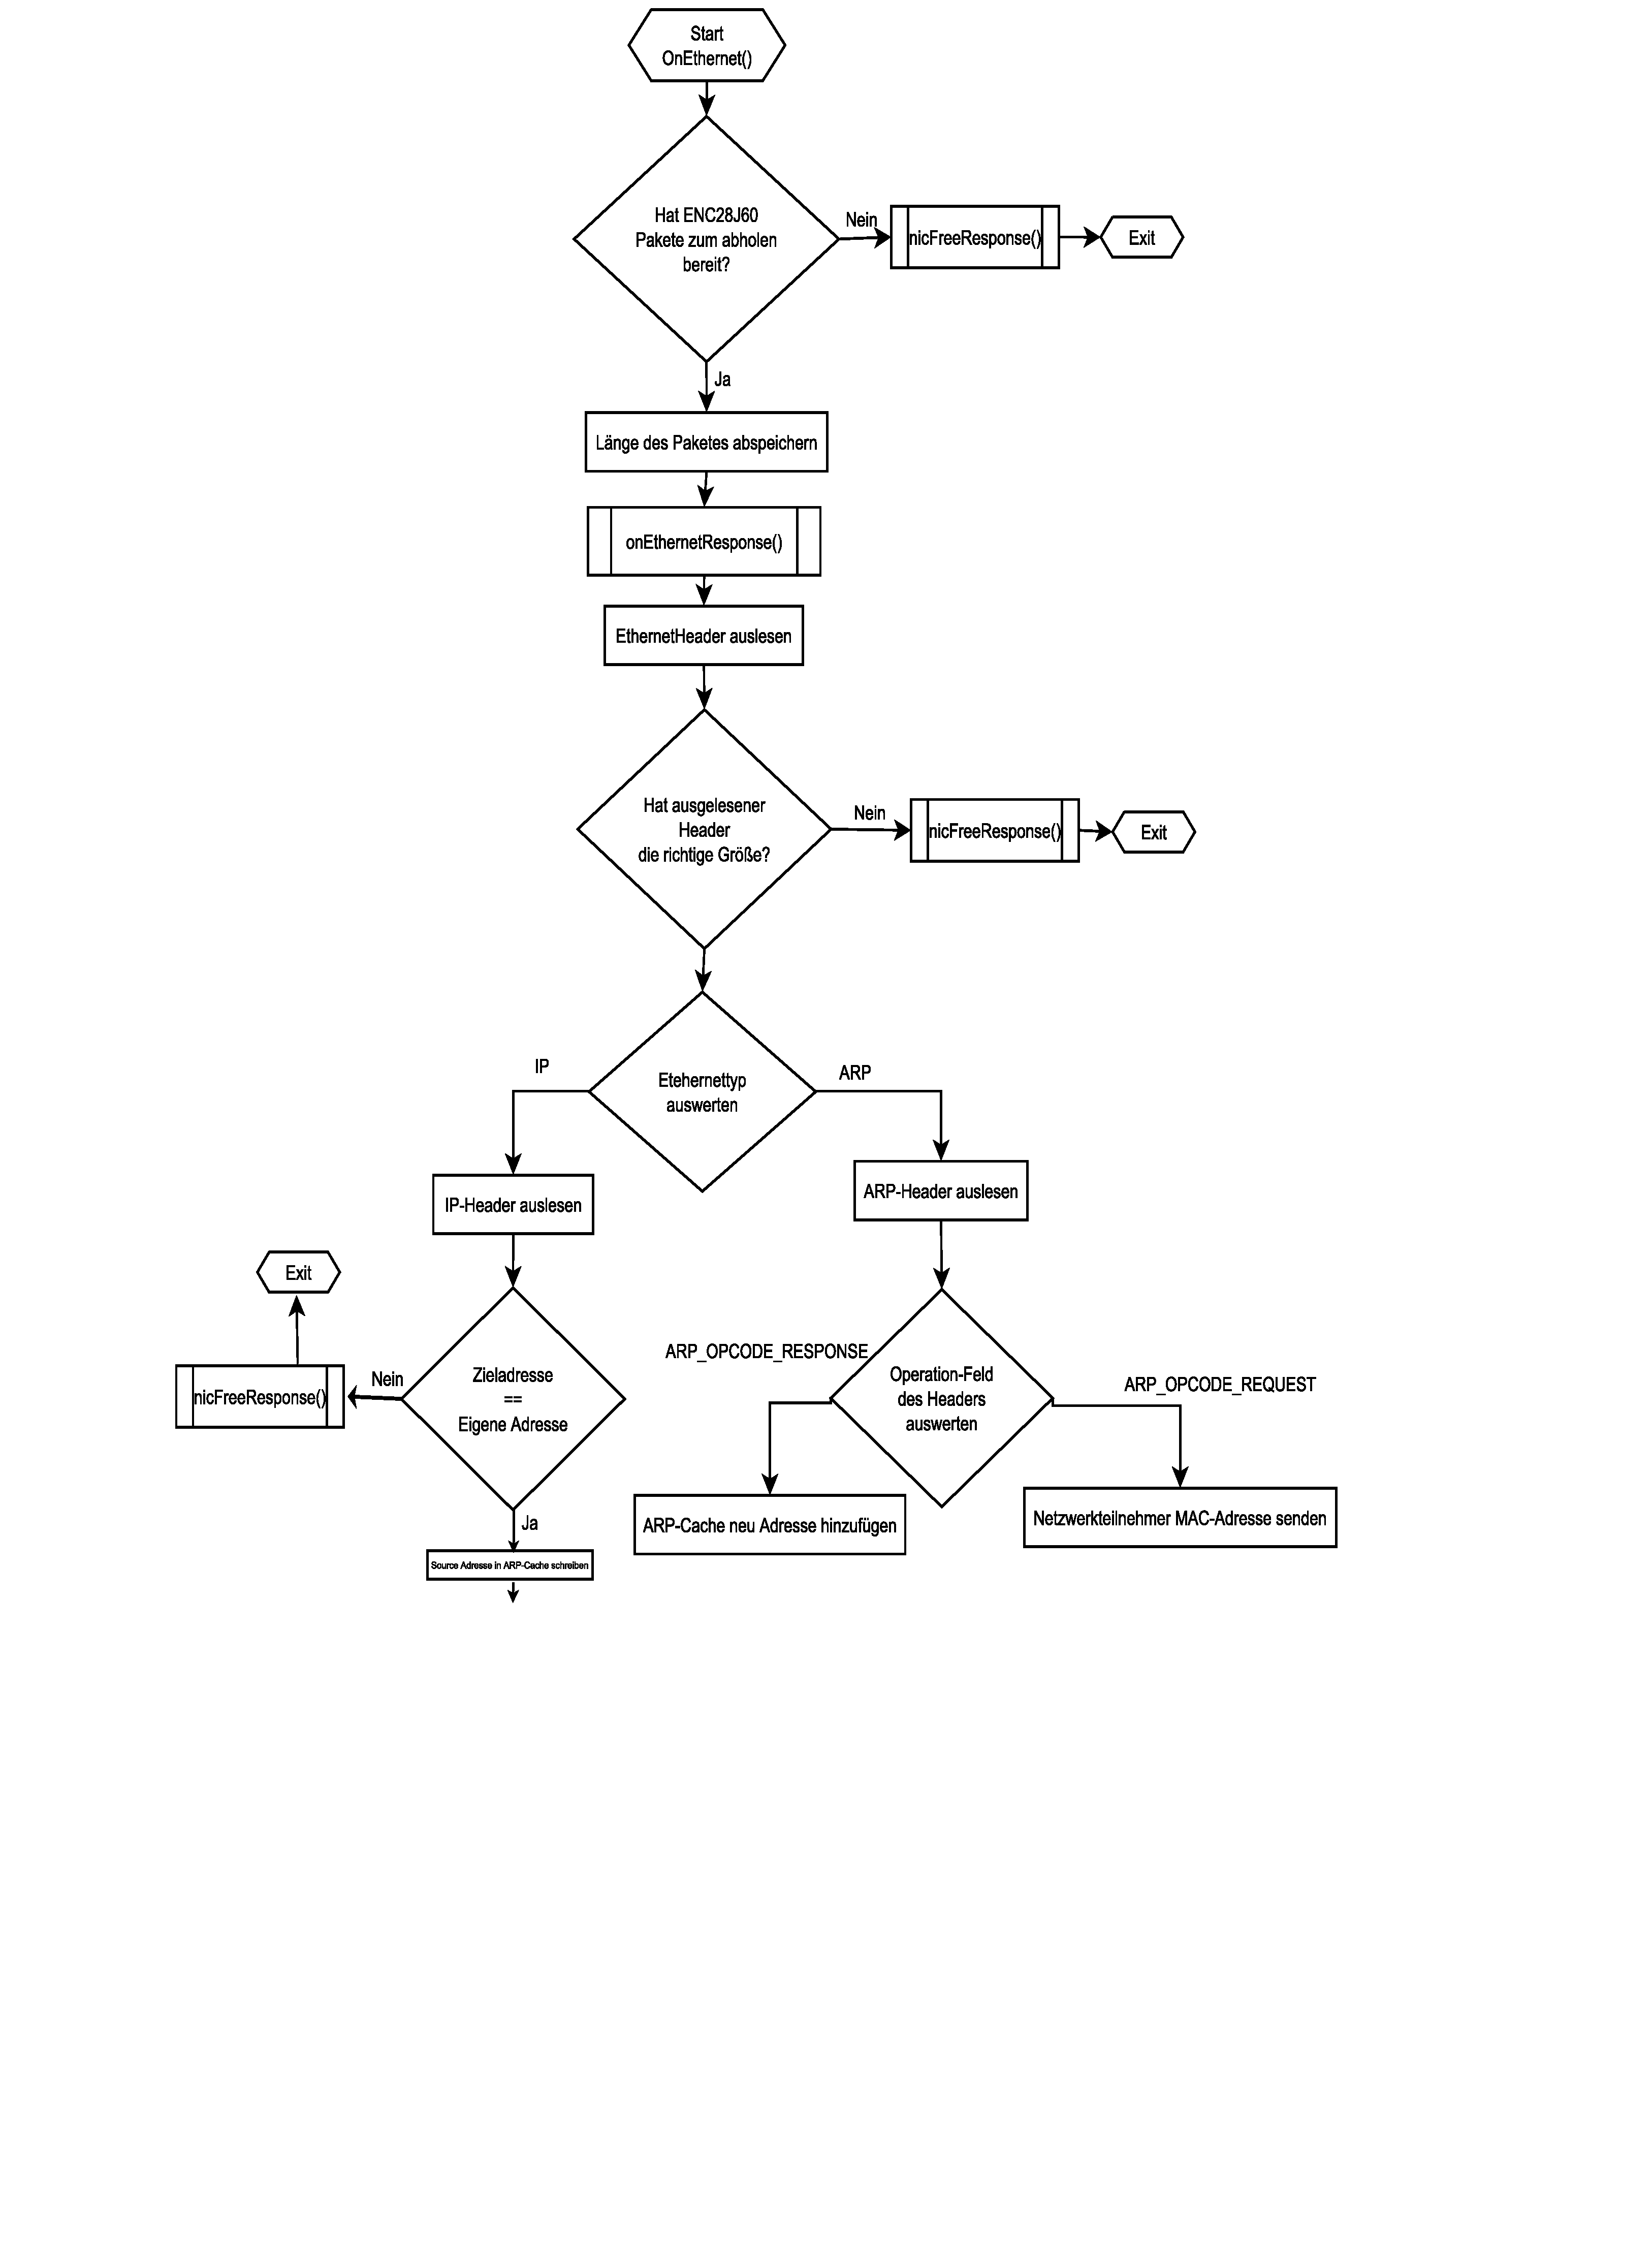
\includegraphics[width=0.8\textwidth]{figures/ethernetto232-dia-01.eps}
	\caption[Empfang eines Ethernet-Paketes]{Empfang eines Ethernet-Paketes}
	\label{fig:ethernettors232 part1}
\end{figure}

\begin{figure}[H]
	\centering
	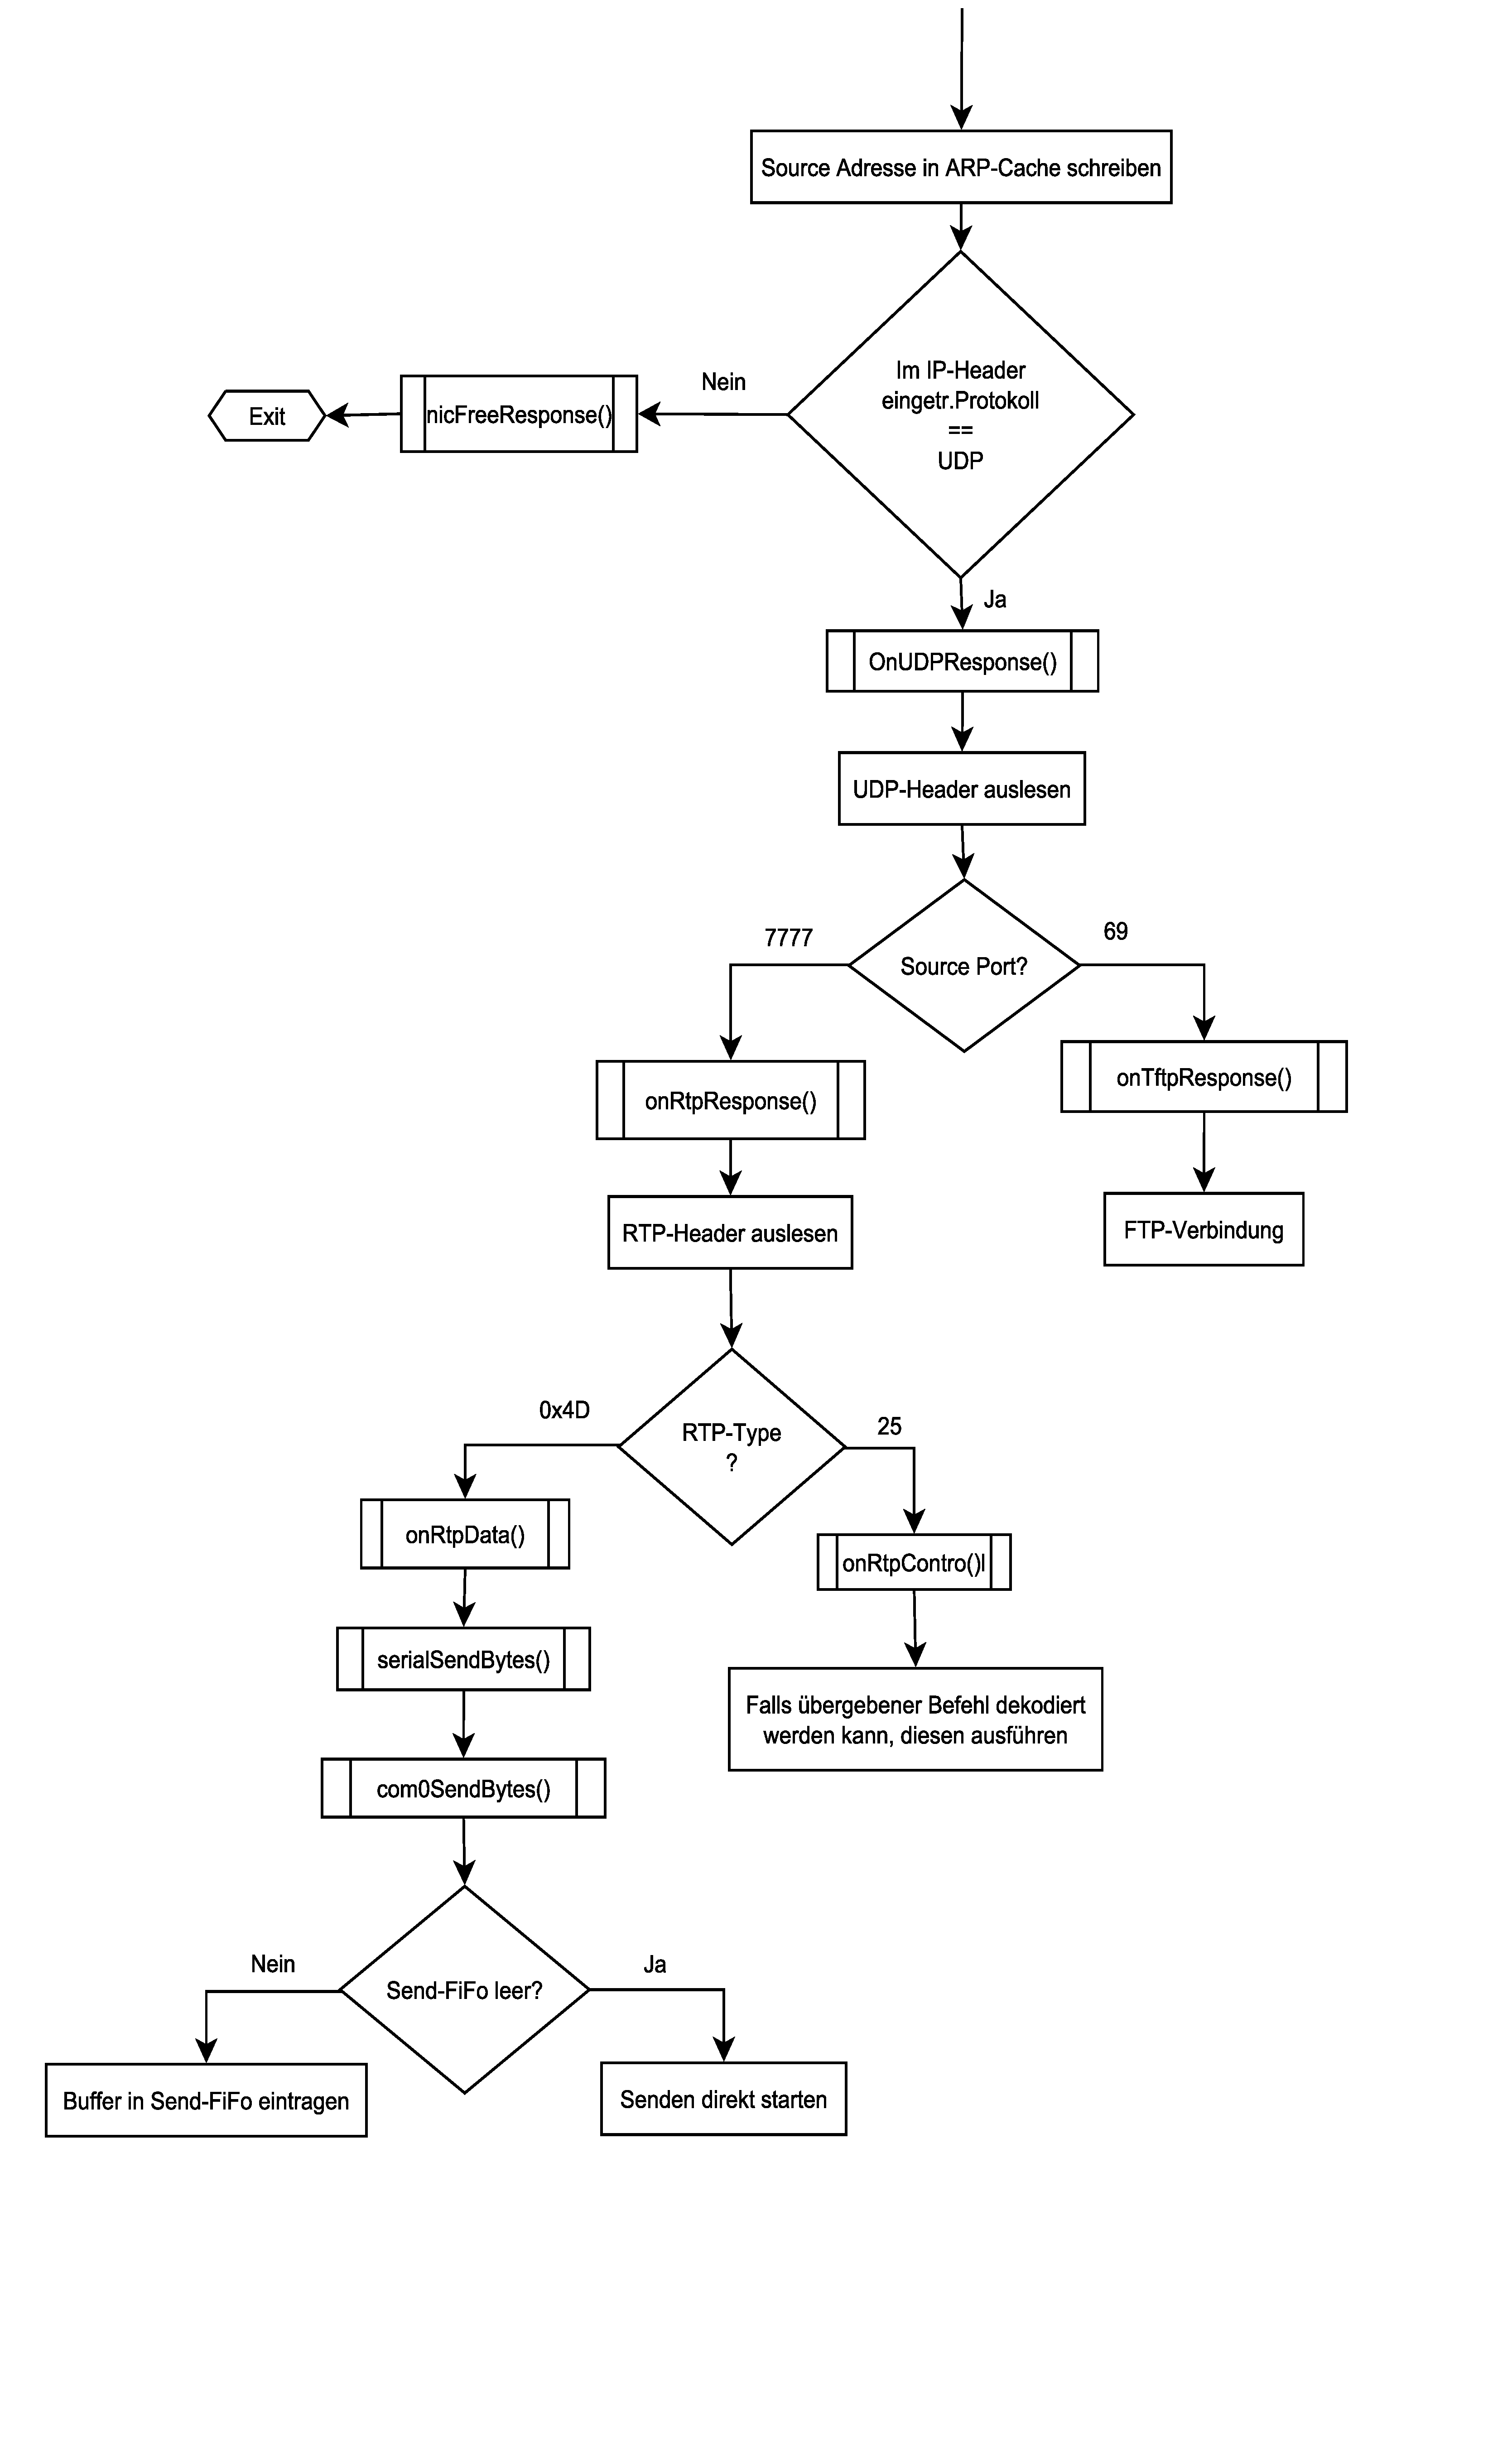
\includegraphics[width=0.8\textwidth]{figures/ethernetto232-dia-02.eps}
	\caption[Empfang eines Ethernet-Paketes]{Empfang eines Ethernet-Paketes}
	\label{fig:ethernettors232 part2}
\end{figure}




\subsection{Timer und Echtzeitverhalten}
\subsubsection{Realisierung beim Messadapter}
Als Timer bezeichnet man eine Variable oder im Falle eines Mikrocontollers ein Register das immer in gleichen Zeitabstnden inkrementiert oder decrementiert wird. Bei  erreichen eines vorher definierten Wertes arbeitet man einen bestimmten Codeabschnitt ab. Der Zeitabschnitt in welchem der Wert gezhlt wird kann in der Regel eingestellt werden und ist meist ein Bruchteil des Systemtaktes. Ein vorher bestimmter Wert kann zum Beispiel ein Overflow des Registers sein und der angesprochene Codeabschnitt eine so genannte ISR (Interrupt Service Routine). Auf diese Weise lsst sich Interruptgesteuert sehr einfach ein bis mehrere, je nach Mikrocontroller, Timer realisieren. Im Falle des Messadapters wird bereits ein Interrupt beim ankommen von Daten an der RS232 Schnittstelle ausgelst so dass, der Interrupt fr  den Timer und der Interrupt fr ankommende Daten durchaus gleichzeitig auslsen knnten. Im allgemeinen Fall kann bei Mikrocontrollern nicht eingestellt werden welcher Interrupt bevorzugt behandelt wird. Auch wenn der UART mehrere Zeichen, in der Regel 4Byte, zwischenspeichern kann, ist dieser Puffer zu gering  da bei hohem Datenaufkommen das Abarbeiten der Interrupt Routine fr den Timer zu lange dauert. Auch ist so nur eine begrenzte Anzahl an Timern realisierbar. Daher wurde bei dem Messadapter eine andere Realisierung fr die Timer gewhlt. Fr die Timer wurde als Speicherstruktur eine verkettete Liste gewhlt die den Aufbau wie in Abbildung \ref{fig:speicherstruktur} hat. Jedes Mal wenn ein Timer hinzugefgt werden soll wird er in die Liste nach dem Wert timebomb sortiert abgelegt.  Der Vorteil bei einer sortierten List ist, dass man bei der Suche nach einem abgelaufenem Timer nicht alle Elemente durchlaufen werden mssen sondern nur das erste Element betrachtet werden muss. Zustzlich zu dieser Speicherstuktur wird eine globale Variable overflows durch einen Interrupt inkrementiert, dies ist betreffend Datenverlust nicht kritisch da hier nur ein Befehl ausgefhrt wird und dann wieder zum ursprnglichen Programmablauf zurckgegangen wird. Der Interrupt ist so konfiguriert das overflows 4 mal pro Sekunde inkrementiert wird. ber die Funktion rtcGetTime64() wird  der Wert von overflow in ms umgerechnet zurckgegeben, womit man zu jeder Zeit abfragen kann wie lange in Millisekunden der Mikrocontroller bereits luft. Nun wird bei jedem zyklischen Durchlauf der main-Methode die Funktion onTimer() aufgerufen. Die Funktion onTimer berprft ob vom ersten Element in der geordneten Liste der eingetragene Zeitwert erreicht wurde oder nicht. Falls dieser erreicht wurde wird die Adresse der Funktion, welche in der Variable callback in jedem TimerElement gespeichert wird, zwischengspeichert. Daraufhin wird, um keinen Speicherplatz zu verlieren, das komplette TimerElement gelscht. Jetzt kann die zum abgelaufenen Timer gehrende Callback-Funktion aufgerufen werden. Soll ein Timer kontinuiertlich nach einer bestimmten Zeitspanne auslsen muss in der Callback-Funktion ein neues TimerElement erstellt werden.
Mit dieser Technik knnen keine hochprzisen Timer realisert werden, da ein ablaufen eines Timers immer erst in der Funktion onTimer() bemerkt wird. Da bei dem Messadpater kein preemptives Scheduling verwendet  werden soll, ist diese technik ausreichend.


\begin{figure}[H]
	\centering
	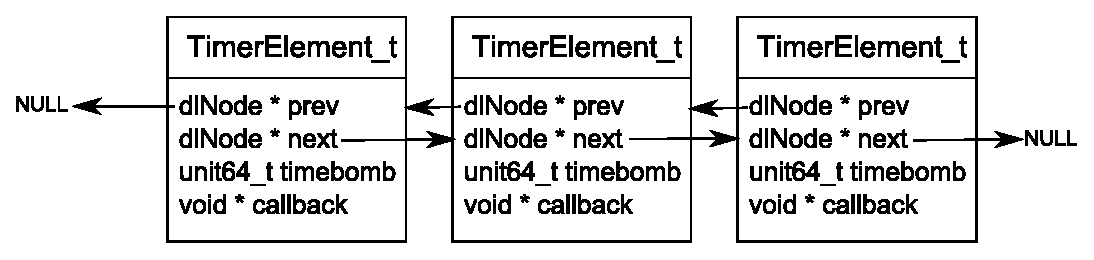
\includegraphics[width=0.8\textwidth]{figures/speicherstrukturtimer.eps}
	\caption[Speicher Struktur der Timer-Liste]{Speicher Struktur der Timer-Liste}
	\label{fig:speicherstruktur}
\end{figure}



\newpage



\subsubsection{Echtzeitverhalten}

Das Echtzeitverhalten des Messadapters hngt stark von der Menge der ankommenden Daten an der seriellen Schnittstelle ab,
da der Sendebuffer sofort per Ethernet gesendet wird falls die 150 Bytes voll sind. Ist die Menge der Daten allerdings eher gering werden die angekommenden Daten im Buffer maximal 500ms Sekunden gehalten und erst dann versendet, was ein erhebliches Delay bedeutet. Das sich ergebene Sendediagramm zeigt Abbildung \ref{fig:sendedia}. Man sieht hier deutlich wann die Pakete aufgrund des Timers bzw. aufrgund des hohen Datenaufkommens versendet werden. Dies ist genau dann der Fall wenn an der RS232 Schnittstelle mehr als 2400Bit/sec anfallen. Dieser Wert berechnet sich aus der Gre des Paketes, welches 150Bytes=1200Bit enthlt, dividiert durch die Zeit welche in unserem Fall eine halbe Sekunde ist.
\newline
\newline

Falls das Datenaufkommen gering ist aber an das Echtzeitverhalten hohe Anforderungen gestellt werden, ist die bisherige Behandlung der Daten eher
unzureichend. Um diese Verzgerung, in der Elektrotechnik beziehungsweise bertragungstechnik auch Jitter genannt, zu verringern wurde die obere Schranke von 150Bytes nicht mehr nur als Konstante im Sourcecode eingegeben sondern liegt als Wert im EEPROM und kann hier flexibel ber den Konfigurationskanal eingestellt werden. Die Befehle zum einstellen sind wie in Tabelle \ref{tab:kommandos} noch erwhnt: "`:setSendLimit X?"' und "`:getSendLimit?"'.
Wenn der Wert jetzt auf 30Byts gestellt wird und es nur ein geringes Datenaufkommen gibt tritt das maximal auftretende Delay von einer halben Sekunde wesentlich seltener auf daher der Jitter wurde also verringert.



\begin{figure}[H]
	\centering
	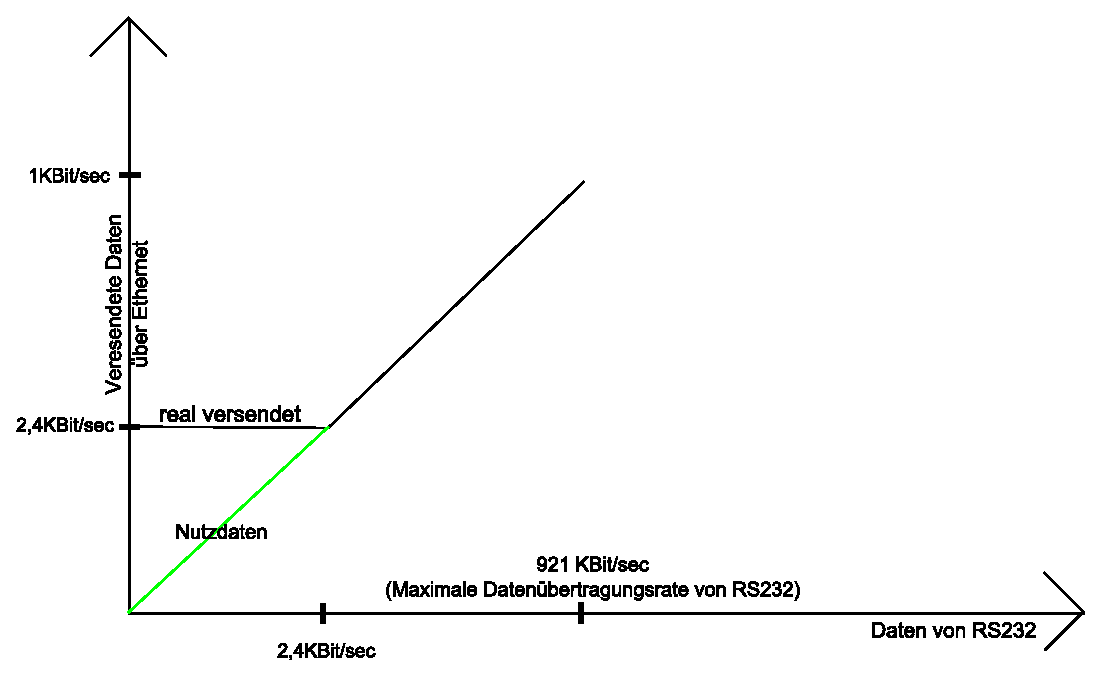
\includegraphics[width=0.8\textwidth]{figures/sendeverhalten.eps}
	\caption[Sendeverhalten des Messadapters]{Sendeverhalten des Messadapters}
	\label{fig:sendedia}
\end{figure}


\newpage

\section{Konfiguration und Debugging}

\subsubsection{Konfiguration}

\label{chapter:konfig}

Da der Messadapter universell verwendet werden soll und man sich nicht schon beim programmieren des Mikrocontrollers sich fr eine Messumgebung entscheiden mssen soll, wurde der Messadapter so erstellt das man seine Konfiguration jederzeit beliebig ndern kann.
So kann zum einen bei der RS232-Schnittstelle jede Datenrate eingestellt oder auch die Anzahl der Daten- und Stopbits flexibel konfiguriert werden. Auch ist es mglich die Adresse und den Destination Port des Zielrechners fr Daten im Betrieb zu ndern sowie die Mac-Adresse oder den Source-Port fr die Pakete zum versenden. All dies kann einmal ber die ttyS1 (RS232) oder auch ber das Ethernet geschehen. Dazu wird im Identifier des RTP-Headers festgehalten um was fr eine Art von Paket es sich handelt und dann entweder an die ttyS0(RS232)  wieder ausgegeben oder aber es wird der Konfigurationsbefehl vom Mikrocontroller dekodiert und umgesetzt. Falls Daten an der ttyS1-Schnittstelle ankommen werden diese Daten immer als Konfigurationsbefehle interpretiert. Dazu wurden von Martin Schwarz im Rahmen seiner Studienarbeit diverse Befehle erstellt und von mir um die folgenden Befehle noch erweitert.

\vspace{1 cm}

\begin{table}[H]

\caption[Kommando-bersicht]{Kommando-bersicht}
\label{tab:kommandos}

\begin{tabular}[H]{llll}\toprule
Befehlsname  & Parameter   							& Kommentar und Beispiel\\ \midrule
getParity    &   												& :getParity? Gibt die Paritt (siehe Tabelle \ref{parity}) zurck   \\
setParity    & Paritt								  & :setParity 2? Setzt Paritt auf : Enabled, Even Parity     \\
\hline
getStopBits  & 											    & :getStopBits? Gibt die Anzahl der Stopbits zurck   \\
setStopBits  & Anzahl Stopbits					& :setStopBits 1? Setz die Anzahl der Stopbits auf 1 \\ 
\hline
getDataBits  &  												& :getDataBits? Gibt die Anzahl der Datenbits zurck \\ 
setDataBits  & Anzahl Datenbits 				& :setDataBits 7? Setzt die Anzahl der Datenbits auf 7\\ 
\hline
getSendLimit  &  												& :getSendLimit? Gibt an ab welcher Datenmenge der\\
							&													&  Sendbuffer versendet wird \\ 
setSendLimit  & Anzahl Datenbits 				& :setSendLimit 60? Setzt die Gre des \\
							&													&  Sendebuffer-Limits auf 60Bytes\\ 
\hline
getConfig    & 													& :getConfig? Liefert Gesamtkonfig. Siehe \ref{fig:getconfig}  \\ \bottomrule
\end{tabular}
\end{table}


\vspace{1 cm}


\begin{table}[H]

\caption[Parity]{Parity}
\label{parity}

\centering
\begin{tabular}[H]{llll}\toprule
Parity  & Parity Modus \\ \midrule
0    		& Disabled \\
1    		& Enabled\\
2  			& Enabled, Even Parity \\
3  			& Enabled, Odd Parity\\ \bottomrule

\end{tabular}

\end{table}



\vspace{1 cm}

\begin{figure}[H]
	\centering
	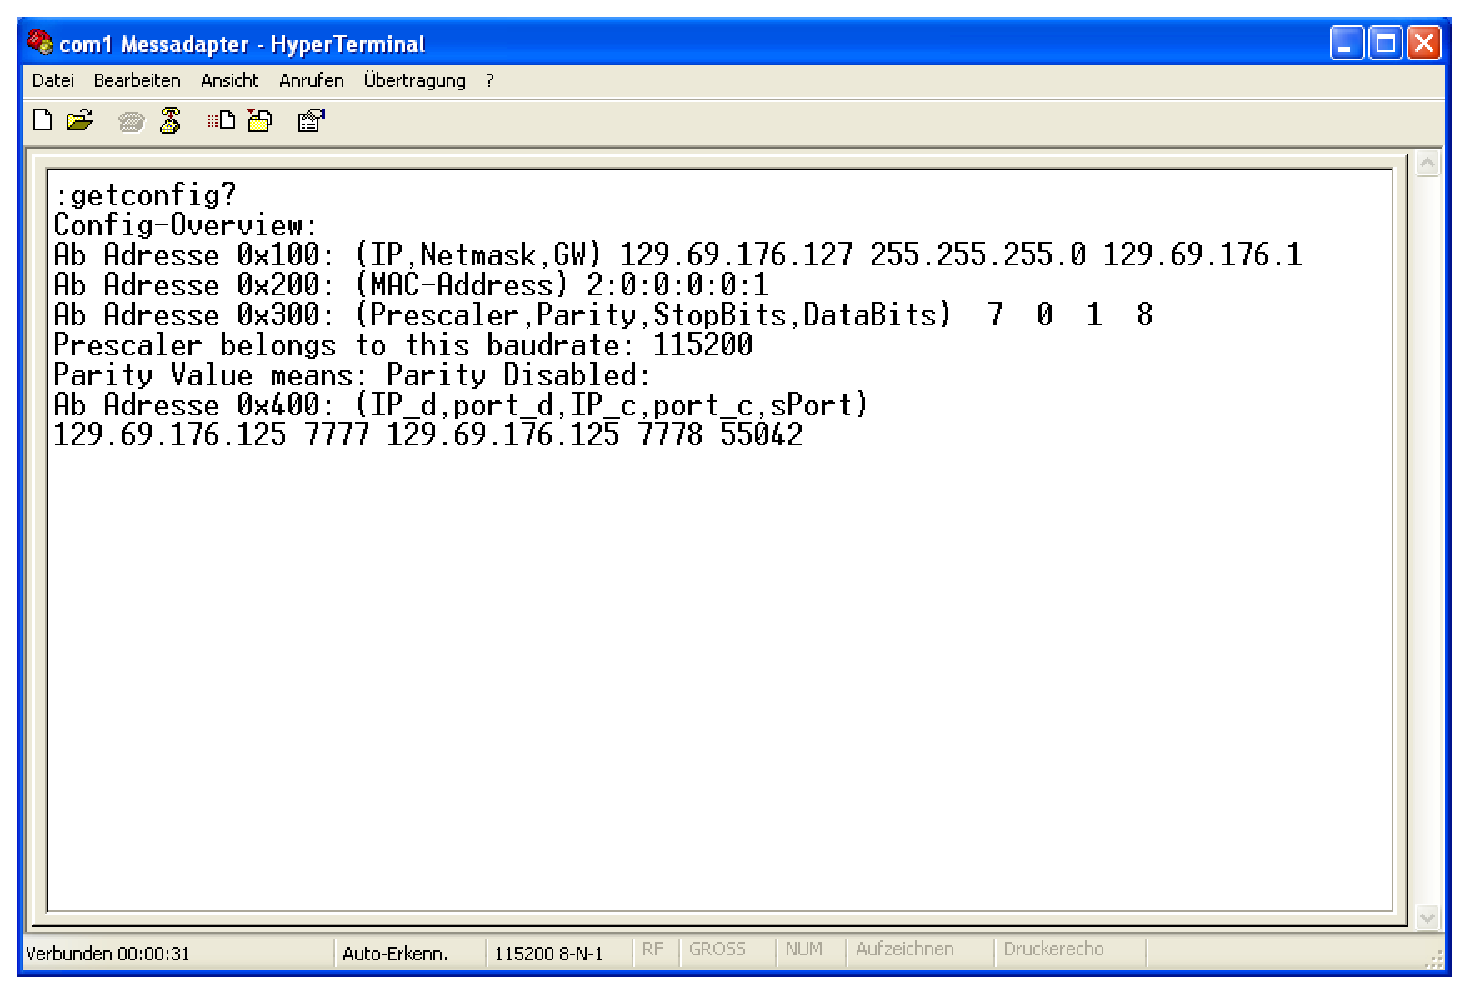
\includegraphics[width=1.0\textwidth]{figures/getconfig.eps}
	\caption{Gesamtkonfiguration}
	\label{fig:getconfig}
\end{figure}

\vspace{1 cm}

Der Befehl "`setBaud X "` setzt wie in \ref{tab:kommandos} bereits beschreiben die Baudrate. Dabei wird nach der Dekodierung des Befehls zunchst
geprft ob es sich hier um eine gltige Baudrate handelt. Ist diese berprfung positiv wird im EEROM an der entsprechenden Stelle der neue Wert
eingetragen. Nach einem Neustart des Messadapters wird der Wert dann wieder eingelesen und die eingegebene Baudrate benutzt.
Was ein EEPROM ist und welche Werte hier vom Messadapter noch gespeichert werden wird in \ref{chp:eeprom} beschrieben.

\vspace{1 cm}
\begin{figure}[H]
	\centering
	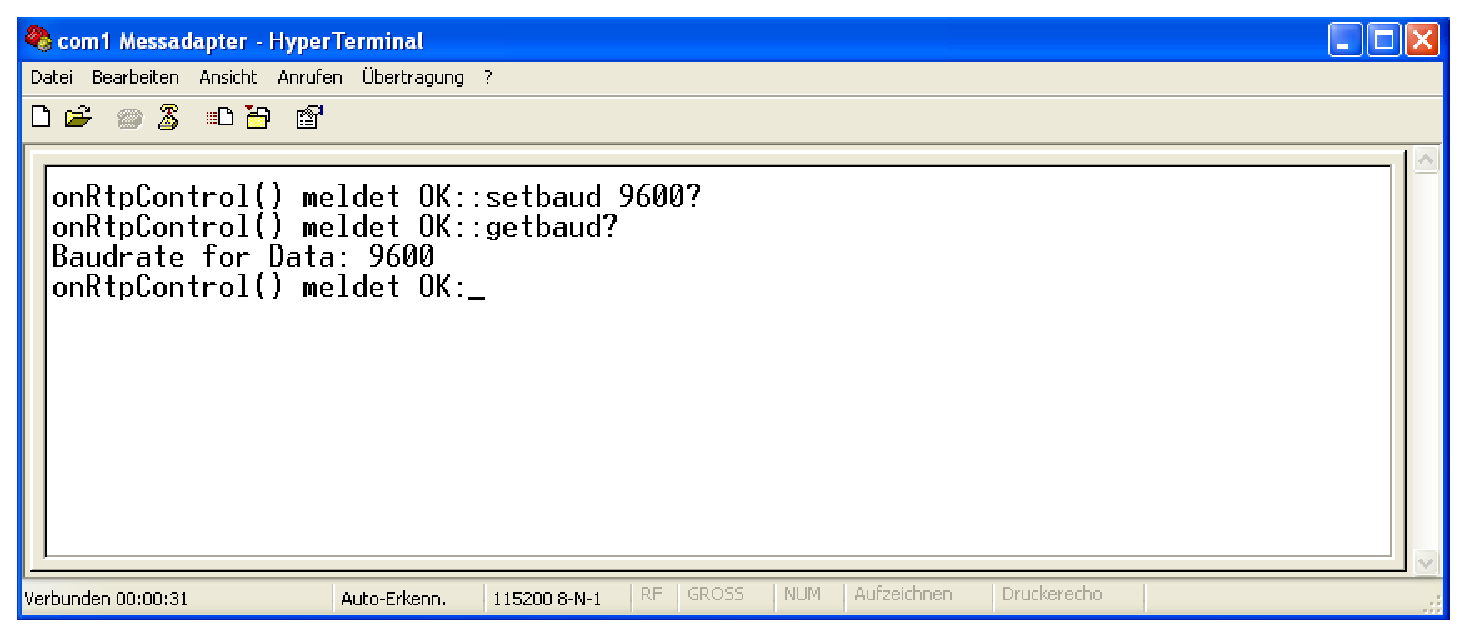
\includegraphics[width=1.0\textwidth]{figures/setbaud.eps}
	\caption{Beispiel: Setzen eines Wertes (Baudrate) im EEPROM}
	\label{fig:setBaud}
\end{figure}
\vspace{1 cm}




\subsubsection{EEPROM} 
\label{chp:eeprom}

EEPROM (engl. Abk. fr electrically erasable programmable read-only memory, wrtlich elektrisch lschbarer programmierbarer Nur-Lese-Speicher) ist ein nichtflchtiger, elektronischer Speicherbaustein, der hufigen Einsatz in eingebetteten Systemen findet, auch gngige Mikrocontroller wie die der ATMega-Reihe besitzen durchgngig interne EEPROM-Speicher.
EEPROMs knnen byteweise beschrieben und gelscht werden.
FlashEEPROMs bentigen zwischen 1s und 1 ms fr einen Schreibzyklus, wohingegen herkmmliche EEPROMs mit 1 ms bis 10 ms erheblich langsamer sind. Daher verwendet man EEPROMS bevorzugt, wenn einzelne Datenbytes in greren Zeitabstnden verndert und auch ohne Spannungs-Strom-Versorgung weiter gespeichert werden mssen, wie zum Beispiel bei den Konfigurationsdaten des Messadapters. Es werden alle 
Konfigurationsdaten im EEPROM gespeichert die fr den Einsatz des Messadapters wichtig sind. So werden Einstellungen wie die Baud-Rate der RS232-Schnittstelle oder die IP-Adresse des Netzwerkcontrollers nur selten gendert was den EEPROM dazu prdestiniert hierfr verwendet zu werden. 
Der Messadapter legt seine Daten wie in Abbildung \ref{fig:eeprom} zu sehen ist ab.
Ab der Adresse 0x100 liegen Daten die mit der Konfiguration des Netzwerkcontrollers zu tun haben, auer der Mac-Adresse welche ab der Adresse 0x200 abgelegt ist. Ab der Adresse 0x300 liegen dann alle bentigten Informationen um eine Verbindung ber die RS232-Schnittstelle aufzubauen. Ab 0x400 sind dann noch nacheinander die Adressen der Zielrechner einmal fr den Daten und zum anderen fr 


\begin{figure}[H]
	\centering
	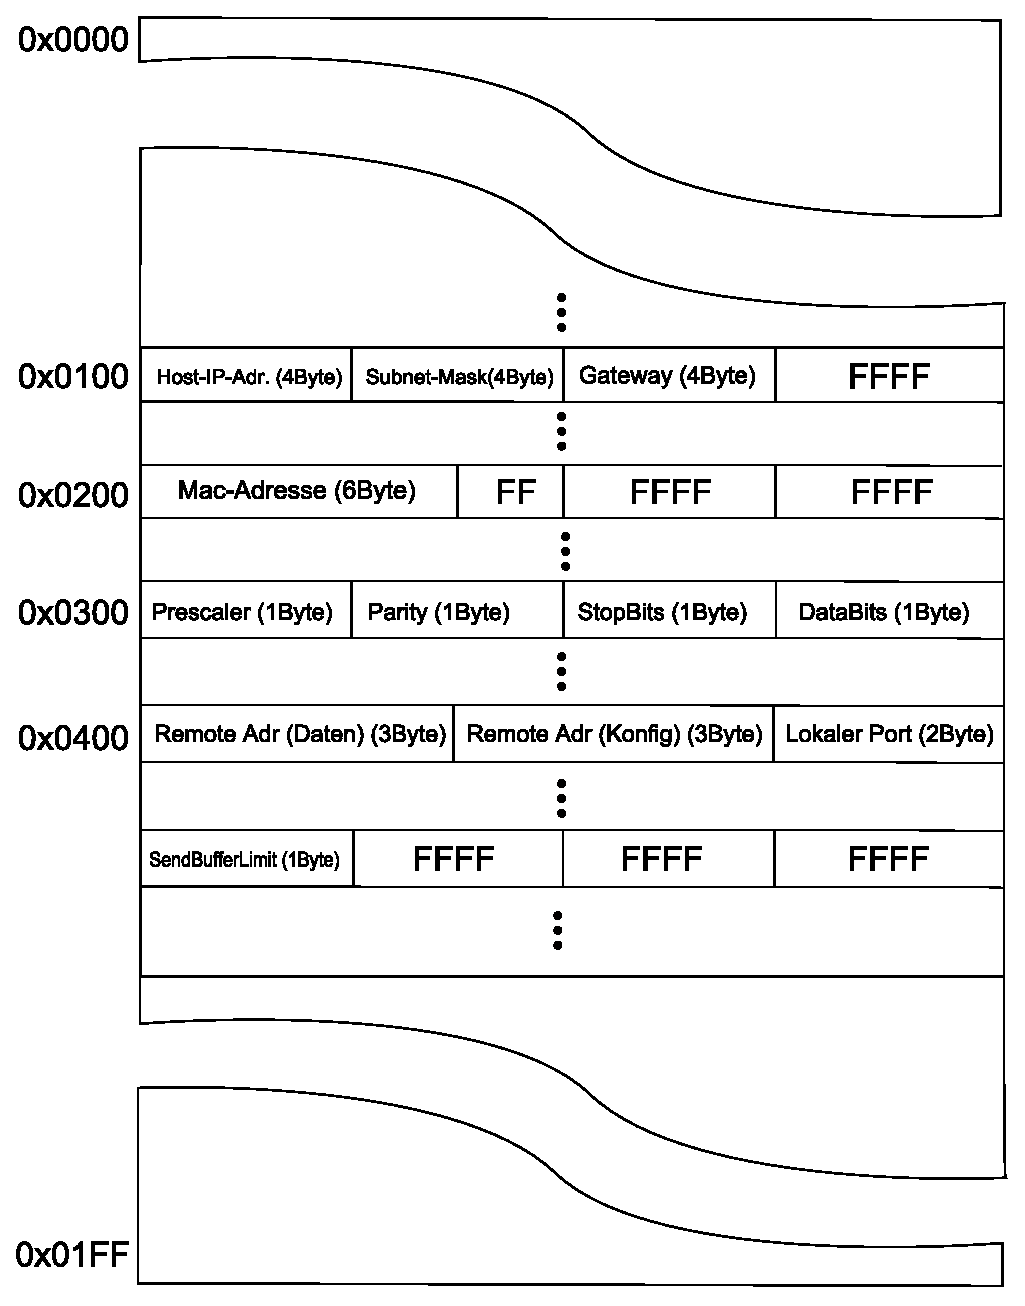
\includegraphics[width=0.8\textwidth]{figures/eeprom-belegung.eps}
	\caption[Eeprom Belegung]{Eeprom Belegung}
	\label{fig:eeprom}
\end{figure}





\subsubsection{Debugging ber COM-Schnittstelle (ttyS1)}

hier noch ein Bild das da eine zweite COM ist

Beim Debugging wir der Vorgang in der Softwareerstellung benannt bei dem es darum ein ausgemachtes Fehlverhalten(Bug) zu lokalisieren. Dabei gibt es verschiedene Vorgehensweisen die wohl am effektivsten und am lngsten dauernde ist die den Code zeilenweise ausfhren zulassen und dabei die Werte der Variablen zu betrachten. Dies ist nicht nur bei Software fr den Computer mglich sondern auf auch fr Mikrocontroller. Eine Mglichkeit ist es einen Debugger zu benutzen. Bei Mikrocontrollern von AVR kommt hier der JTAG in frage mit dessen Hilfe kann die Taktrate des Mikrocontrollers herabgesetzt werden und der Code Schritt fr Schritt durchlaufen werden. Allerdings ist dies nicht bei bei jeder Softwareart praktikabel, beim Messadapter zum Beispiel luft alle 50ms ein Timer ab. Will man jetzt den Code debuggen springt der Debugger stndig nur in den Code der durch den Timer ausgefhrt wird. Daher kann beim Messadapter die Kommunikationsschnittstelle ttyS1 (RS232) nicht nur zum konfigurieren benutzt werden sondern es knnen auch an bestimmten Stellen im  Programm Meldungen abgegeben werden. Damit kann geprft werden ob ein bestimmter Codeabschnitt berhaupt ausgefhrt wird oder welchen Wert eine Variable zu welchem Zeitpunkt annimmt. Ein Beispiel bei welchem diese Verfahren erfolgreich angewandt wurde ist als Fehler beim Senden eines Paketes gesucht. Deshalb wurde in allen beteiligten Funktionen ein Funktionsaufruf zum debuggen integriert. Als Ergebnis kam dann die Antwort welche in Abbildung \ref{fig:debug-ausgabe} dargestellt ist. Man sieht hier, dass alle Debugaufrufe aus den Funktionen onSerial(),onCom0RecvBytes(), rtpSendCDPData(), onRtpRequest und onUdpRequest() erfolgreich aufgerufen wurden. In der Funktion onIP4Request() gab es allerdings zwei Debugaufrufe wie in Abbildung \ref{fig:debug-code} zu sehen ist. In dem Debug-Protokoll ist aber nur der erste Aufruf verzwichnet, was bedeutet, dass der Fehler arpLookupMacByIPv4() zu finden war.


\vspace{1 cm}
\begin{figure}[H]
	\centering
	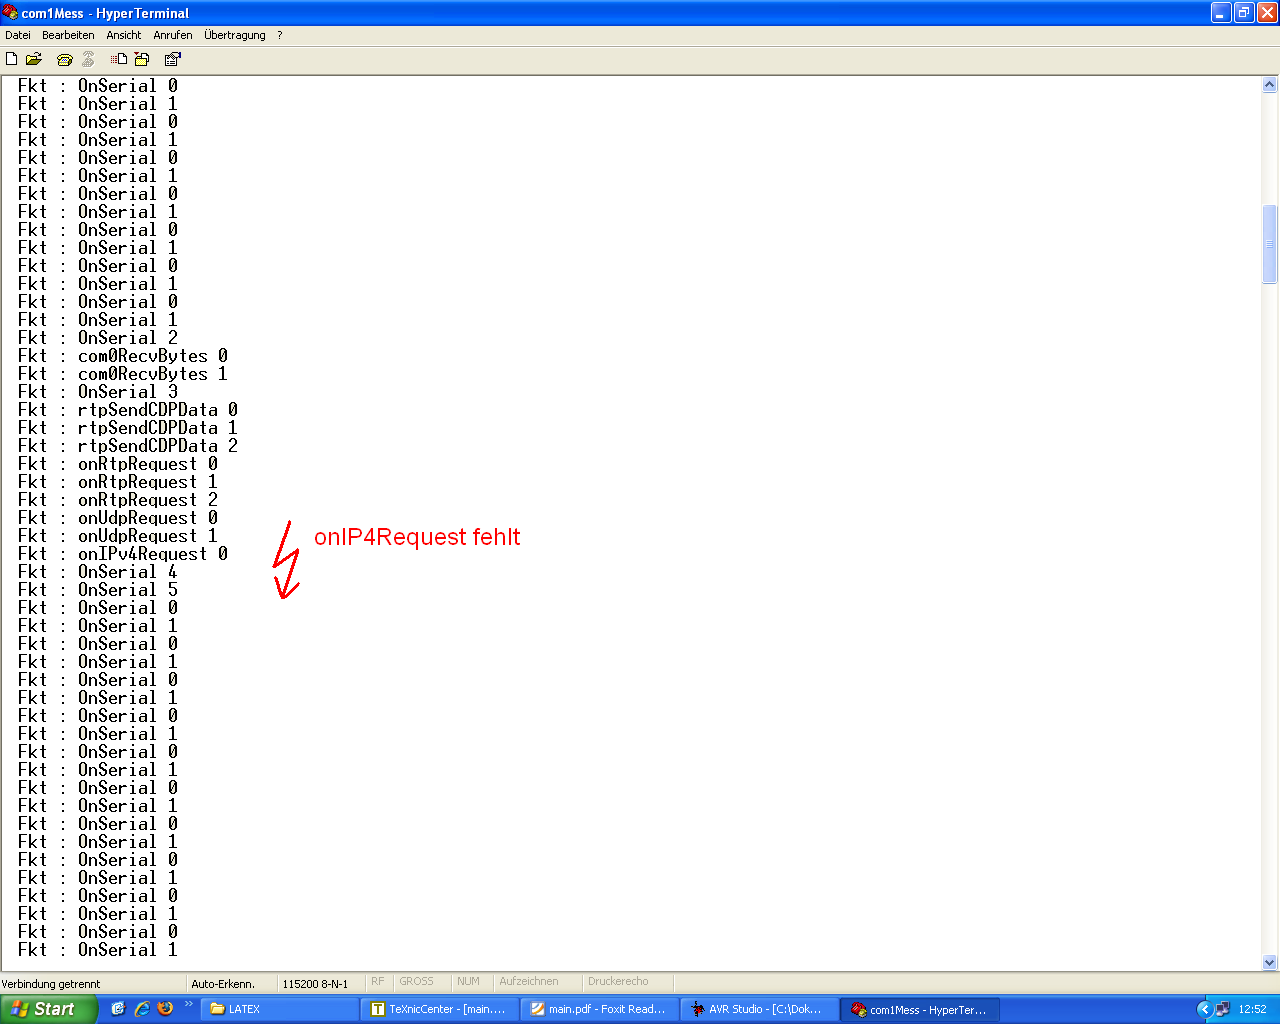
\includegraphics[width=0.6\textwidth]{figures/debugging_ausgabe.eps}
	\caption{Debug-Ausgabe vom Sendeprozess}
	\label{fig:debug-ausgabe}
\end{figure}
\vspace{1 cm}


\vspace{1 cm}
\begin{figure}[H]
	\centering
	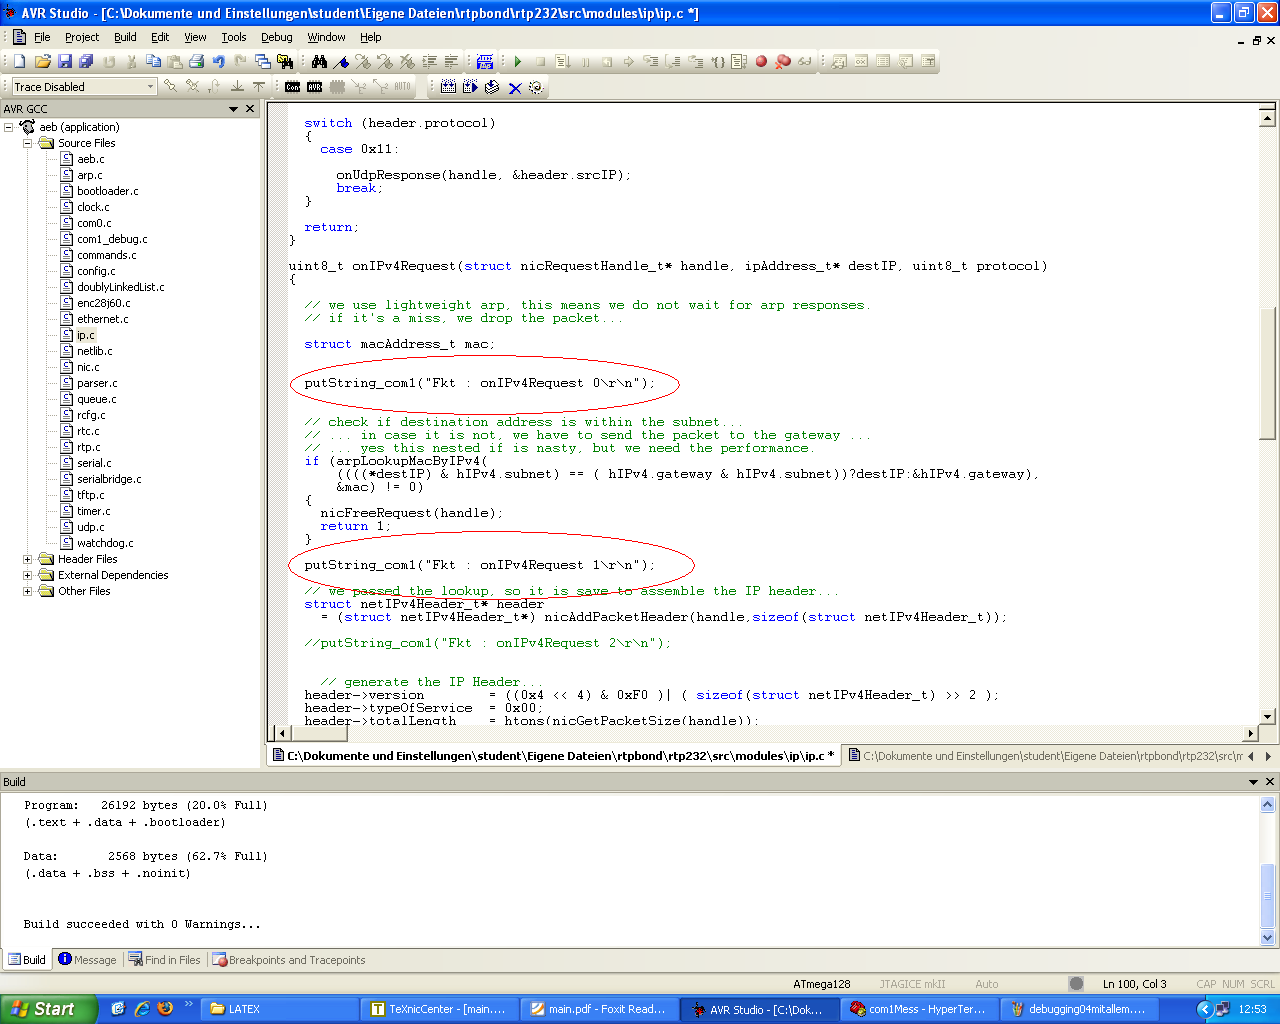
\includegraphics[width=0.6\textwidth]{figures/debugging_code.eps}
	\caption{Debug-Aufrufe}
	\label{fig:debug-code}
\end{figure}
\vspace{1 cm}






\subsubsection{Bootloader}


Mikrocontroller knnen auf verschiedene Art und Weisen programmiert werden. Die am weitesten verbreite Art ist mithilfe eines Programmiergertes (engl.: programmer). Mit diesem Programmiergert knnen entweder ber COM, USB oder auch Bussystemen wie CAN der Programmcode des Mikrocontrollers als Daten bertragen und im Flash werden. Der Nachteil dieser Programmiergerte ist der das diese meist teuer sind und zudem nur speziell fr einige wenige Mikrocontroller hergestellt wurden.
Ein weiter Weg den Mikrocontroller Flash zu beschreiben ist das Programmieren von einem selbst geschriebenen Bootloader. 
Ein Bootloader ist ein Programm, dass in einem bestimmten Speicherbereich (Boot Loader Flash Section) liegt. Im falle eines Neustarts des Mikrocontroller erwartet dieser ein bestimmtes Ereignis wie zum Beispiel: Das Drcken eines Schalters oder bestimmte Daten ber eine Kommunikationsschnitstelle wie der RS232 oder im Falle des Messadapters auf Daten vom Netzwerkcontroller kommend. Falls dieses Ereignis nicht eintritt wird der Mikrocontroller normal gestartet. Der Bootloader bekommt den Programmcode wiederum von Kommunikationsschnittstellen wie COM, USB, CAN oder auch von Speichermedien wie SD-Karten oder MMC Karte.
Bei dem Messadapter wurde als Datenquelle das Netzwerk genommen. Das bedeutet, dass der Bootloader eine Netzwerkverbindung, in diesem Fall FTP-Verbindung,  aufnimmt und den Programmcode neuschreibt. Hier kann allerdings ein Problem auftreten, nmlich dann wenn der Bootloader sich selber berschreiben wrde. Dieses Problem wird bei heutigen Mikrocontrollern derart gelst, dass der Flashspeicher in zwei Bereiche aufgeteilt wird.




\begin{figure}[H]
	\centering
	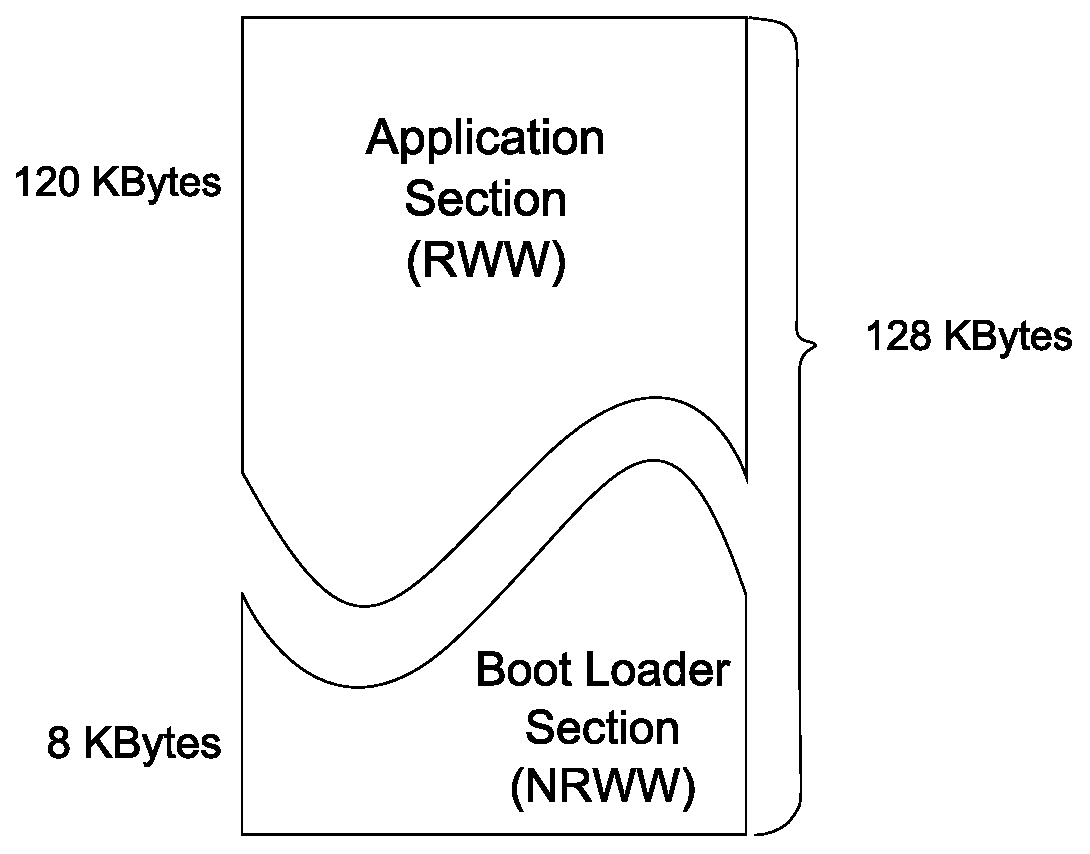
\includegraphics[width=1.0\textwidth]{figures/flashmemory.eps}
	\caption[Beispiel Aufbau des Flash-Memory anhand des ATMega128]{Beispiel Aufbau des Flash-Memory anhand des ATMega128}
	\label{fig:flash}
\end{figure}





Es gibt zum einen den Bereich fr den Programmcode der Anwendung (Application Flash Section) und zum anderen den Bereich fr den Bootloader (Boot Loader Flash Section). 
Dies erffnet die Mglichkeit, den Programm-Flash whrend der Laufzeit vom Bootloader aus zu manipulieren.
In dem Programmablaufplan \ref{fig:bootloader} ist zu sehen wie der Bootloader sich in das gesamte Programm des Mikrocontrollers einfgt. Zunchst wird ein Timer erstellt der nach 10 Sekunden ausgelst wird. Falls der Timer auslst werden ab diesem Zeitpunkt keine FTP-Verbindungen mehr angenommen. Falls vor diesen 10 Sekunden eine FTP-Verbindung zu dem Messadapter hergestellt wird, muss zunchst der Timer auer Kraft gesetzt werden. Daraufhin muss unterschieden werden ob die daraufhin ankommenden Pakete Daten fr den Applikation Flash sind oder als Daten im EEPROM abgelegt werden soll. Dies geschieht anhand des im ersten Paket mitgelieferten Dateinamen. Lautet der Dateiname "`"' werden die Daten in den Programmspeicher (Application Section) geschrieben. Lautet er hingegen "`"' wird mit den Daten das komplette EEPROM mit neuen Werten bespielt. Nun werden die Daten der  darauf folgenden Pakete im gewnschten Speicher solange abgelegt bis alle Daten bertragen wurden. Nach Abschluss des Datentransfers fhrt der Mikrocontroller einen Reset durch und startet danach mit der neuen oder aktualisierten Anwendung, bzw. mit der neuen EEPROM-Belegung neu.

\begin{figure}[H]
	\centering
	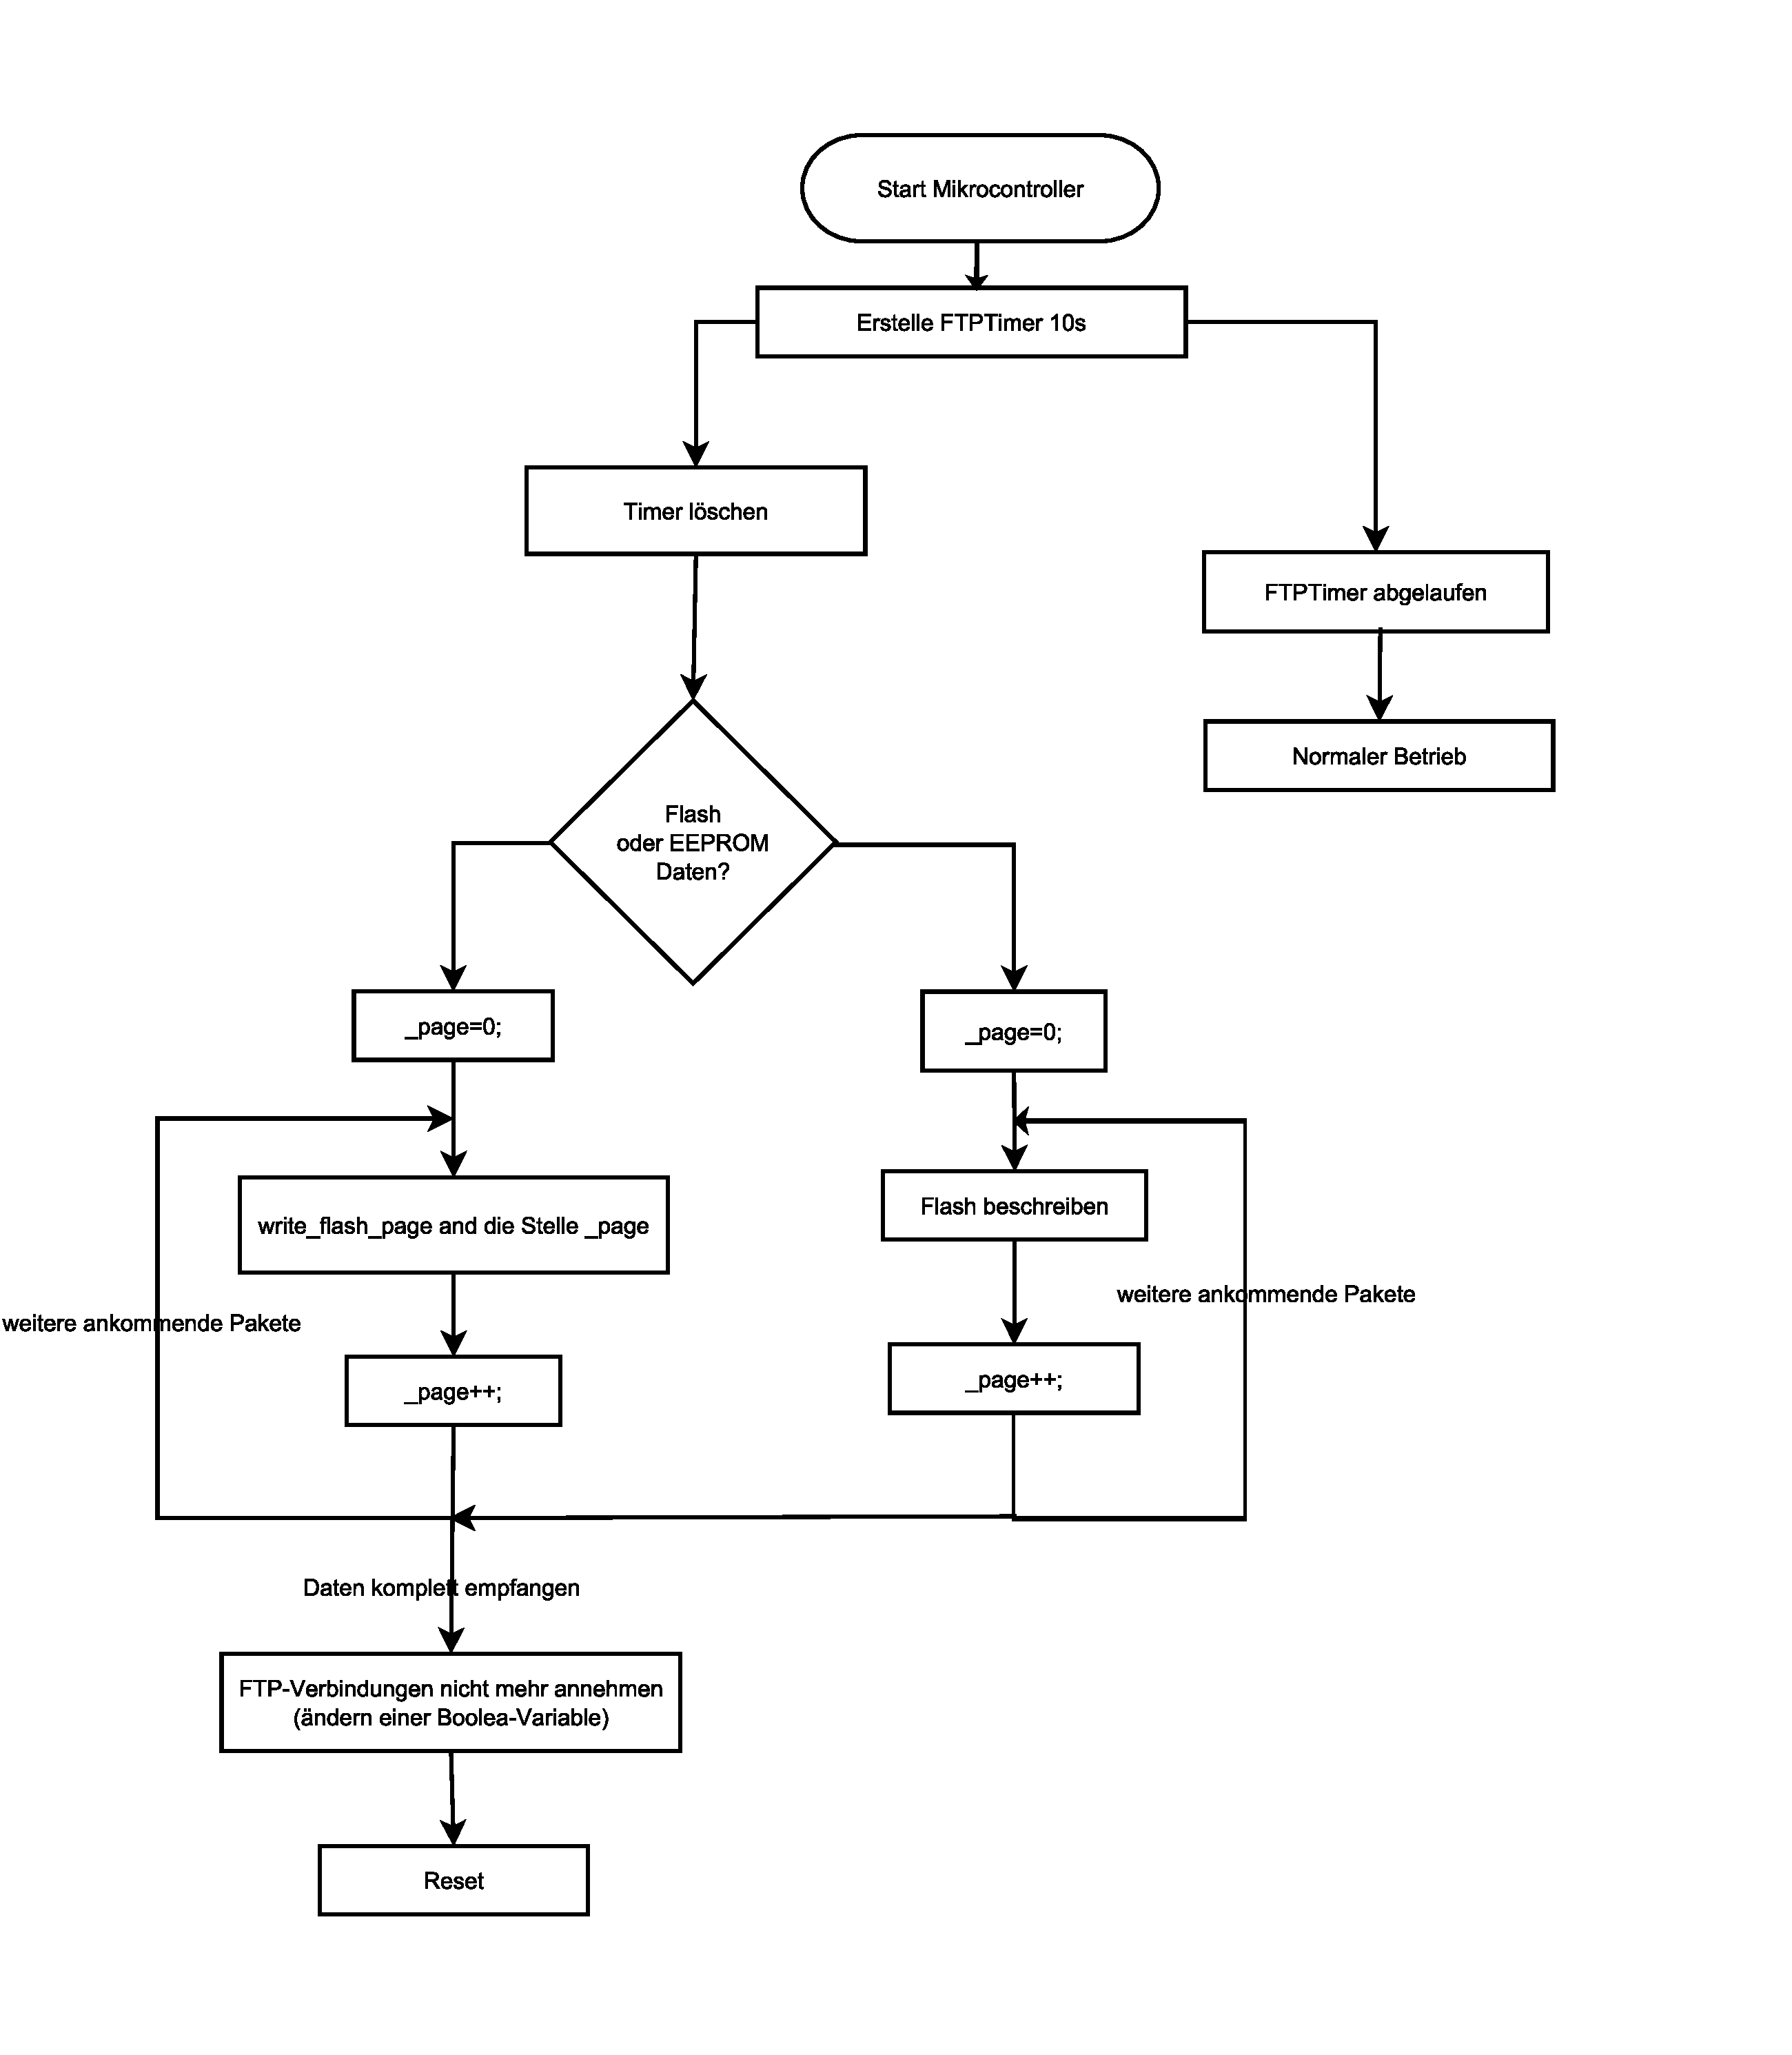
\includegraphics[width=1.0\textwidth]{figures/bootloader.eps}
	\caption[Programmablaufplan des Bootloaders]{Programmablaufplan des Bootloaders}
	\label{fig:bootloader}
\end{figure}



\chapter{Tools and Amendmends}

This is the body (mainmatter) of the Standard LaTeX Book document.

The front matter has a number of sample entries that you should
replace with your own.

Replace this text with the body of your book. Do not delete the
\verb|mainmatter| TeX field found above in a paragraph by itself
or the numbering of different objects will be wrong.

The typesetting specification selected by this document uses the
default class options. There are, however, a number of class
options. The available options include setting the paper size and
the point size of the font used in the body of the document etc.
Details are given as comments right after the \verb|documentclass|
command.

\chapter{The Most Important Features of this Document}

\section{Section}

Use the \verb"\section{Section}" command for major sections, and the
\verb"\subsection{Subsection}" command for subsections, etc.

\subsection{Subsection}

This is just some text under a subsection.

\subsubsection{Subsubsection}

This is just some text under a subsubsection.

\paragraph{Subsubsubsection}

This is just some  text under a subsubsubsection.

\subparagraph{Subsubsubsubsection}

This is just some text under a subsubsubsubsection.

\section{Typesetting Commands}

SSelect a part of the text then click on the button Emphasize (H!), or Bold (Fs), or
Italic (Kt), or Slanted (Kt) to typeset \emph{Emphasize}, \textbf{Bold},
\textit{Italics}, \textsl{Slanted} texts.

You can also typeset \textrm{Roman}, \textsf{Sans Serif}, \textsc{Small Caps}, and
\texttt{Typewriter} texts.

You can also apply the special, mathematics only commands $\mathbb{BLACKBOARD}$
$\mathbb{BOLD}$, $\mathcal{CALLIGRAPHIC}$, and $\mathfrak{fraktur}$. Note that
blackboard bold and calligraphic are correct only when applied to uppercase letters A
through Z.

You can apply the size tags -- Format menu, Font size submenu -- {\tiny tiny},
{\scriptsize scriptsize}, {\footnotesize footnotesize}, {\small small}, {\normalsize
normalsize}, {\large large}, {\Large Large}, {\LARGE LARGE}, {\huge huge} and {\Huge
Huge}.

You can use the \verb"\begin{quote} etc. \end{quote}" environment for typesetting
short quotations. Select the text then click on Insert, Quotations, Short Quotations:

\begin{quote}
The buck stops here. \emph{Harry Truman}

Ask not what your country can do for you; ask what you can do for your
country. \emph{John F Kennedy}

I am not a crook. \emph{Richard Nixon}

I did not have sexual relations with that woman, Miss Lewinsky. \emph{Bill Clinton}
\end{quote}

The Quotation environment is used for quotations of more than one paragraph. Following
is the beginning of \emph{The Jungle Books} by Rudyard Kipling. (You should select
the text first then click on Insert, Quotations, Quotation):

\begin{quotation}
It was seven o'clock of a very warm evening in the Seeonee Hills when Father Wolf woke
up from his day's rest, scratched himself, yawned  and spread out his paws one after
the other to get rid of sleepy feeling in their tips. Mother Wolf lay with her big gray
nose dropped across her four tumbling, squealing cubs, and the moon shone into the
mouth of the cave where they all lived. ``\emph{Augrh}'' said Father Wolf, ``it is time
to hunt again.'' And he was going to spring down hill when a little shadow with a bushy
tail crossed the threshold and whined: ``Good luck go with you, O Chief of the Wolves;
and good luck and strong white teeth go with the noble children, that they may never
forget the hungry in this world.''

It was the jackal---Tabaqui the Dish-licker---and the wolves of India despise Tabaqui
because he runs about making mischief, and telling tales, and eating rags and pieces of
leather from the village rubbish-heaps. But they are afraid of him too, because
Tabaqui, more than any one else in the jungle, is apt to go mad, and then he forgets
that he was afraid of anyone, and runs through the forest biting everything in his way.
\end{quotation}

Use the Verbatim environment if you want \LaTeX\ to preserve spacing, perhaps when
including a fragment from a program such as:
\begin{verbatim}
#include <iostream>         // < > is used for standard libraries.
void main(void)             // ''main'' method always called first.
{
 cout << ''This is a message.'';
                            // Send to output stream.
}
\end{verbatim}
(After selecting the text click on Insert, Code Environments, Code.)


\section{Mathematics and Text}

It holds \cite{KarelRektorys} the following
\begin{theorem}
(The Currant minimax principle.) Let $T$ be completely continuous selfadjoint operator
in a Hilbert space $H$. Let $n$ be an arbitrary integer and let $u_1,\ldots,u_{n-1}$ be
an arbitrary system of $n-1$ linearly independent elements of $H$. Denote
\begin{equation}
\max_{\substack{v\in H, v\neq
0\\(v,u_1)=0,\ldots,(v,u_n)=0}}\frac{(Tv,v)}{(v,v)}=m(u_1,\ldots, u_{n-1})
\label{eqn10}
\end{equation}
Then the $n$-th eigenvalue of $T$ is equal to the minimum of these maxima, when
minimizing over all linearly independent systems $u_1,\ldots u_{n-1}$ in $H$,
\begin{equation}
\mu_n = \min_{\substack{u_1,\ldots, u_{n-1}\in H}} m(u_1,\ldots, u_{n-1}) \label{eqn20}
\end{equation}
\end{theorem}
The above equations are automatically numbered as equation (\ref{eqn10}) and
(\ref{eqn20}).


\section{Lists Environments}

You can create numbered, bulleted, and description lists
(Use the Itemization or Enumeration buttons, or click on the Insert menu
then chose an item from the Enumeration submenu):

\begin{enumerate}
\item List item 1

\item List item 2

\begin{enumerate}
\item A list item under a list item.

\item Just another list item under a list item.

\begin{enumerate}
\item Third level list item under a list item.

\begin{enumerate}
\item Fourth and final level of list items allowed.
\end{enumerate}
\end{enumerate}
\end{enumerate}
\end{enumerate}

\begin{itemize}
\item Bullet item 1

\item Bullet item 2

\begin{itemize}
\item Second level bullet item.

\begin{itemize}
\item Third level bullet item.

\begin{itemize}
\item Fourth (and final) level bullet item.
\end{itemize}
\end{itemize}
\end{itemize}
\end{itemize}

\begin{description}
\item[Description List] Each description list item has a term followed by the
description of that term.

\item[Bunyip] Mythical beast of Australian Aboriginal legends.
\end{description}

\section{Theorem-Like Environments}

The following theorem-like environments (in alphabetical order) are available
in this style.

\begin{acknowledgement}
This is an acknowledgement
\end{acknowledgement}

\begin{algorithm}
This is an algorithm
\end{algorithm}

\begin{axiom}
This is an axiom
\end{axiom}

\begin{case}
This is a case
\end{case}

\begin{claim}
This is a claim
\end{claim}

\begin{conclusion}
This is a conclusion
\end{conclusion}

\begin{condition}
This is a condition
\end{condition}

\begin{conjecture}
This is a conjecture
\end{conjecture}

\begin{corollary}
This is a corollary
\end{corollary}

\begin{criterion}
This is a criterion
\end{criterion}

\begin{definition}
This is a definition
\end{definition}

\begin{example}
This is an example
\end{example}

\begin{exercise}
This is an exercise
\end{exercise}

\begin{lemma}
This is a lemma
\end{lemma}

\begin{proof}
This is the proof of the lemma.
\end{proof}

\begin{notation}
This is notation
\end{notation}

\begin{problem}
This is a problem
\end{problem}

\begin{proposition}
This is a proposition
\end{proposition}

\begin{remark}
This is a remark
\end{remark}

\begin{summary}
This is a summary
\end{summary}

\begin{theorem}
This is a theorem
\end{theorem}

\begin{proof}
[Proof of the Main Theorem]This is the proof.
\end{proof}

\appendix

\chapter{The First Appendix}

The \verb"\appendix" command should be used only once. Subsequent appendices can
be created using the Chapter command.

\chapter{The Second Appendix}

Some text for the second Appendix.

This text is a sample for a short bibliography. You can cite a book by making use of
the command \verb"\cite{KarelRektorys}": \cite{KarelRektorys}. Papers can be cited
similarly: \cite{Bertoti97}. If you want multiple citations to appear in a single set
of square brackets you must type all of the citation keys inside a single citation,
separating each with a comma. Here is an example: \cite{Bertoti97, Szeidl2001,
Carlson67}.

\begin{thebibliography}{9}
\bibitem {KarelRektorys}Rektorys, K., \textit{Variational methods in Mathematics,
Science and Engineering}, D. Reidel Publishing Company,
Dordrecht-Hollanf/Boston-U.S.A., 2th edition, 1975

\bibitem {Bertoti97} \textsc{Bert\'{o}ti, E.}:\ \textit{On mixed variational formulation
of linear elasticity using nonsymmetric stresses and displacements}, International
Journal for Numerical Methods in Engineering., \textbf{42}, (1997), 561-578.

\bibitem {Szeidl2001} \textsc{Szeidl, G.}:\ \textit{Boundary integral equations for
plane problems in terms of stress functions of order one}, Journal of Computational and
Applied Mechanics, \textbf{2}(2), (2001), 237-261.

\bibitem {Carlson67}  \textsc{Carlson D. E.}:\ \textit{On G\"{u}nther's stress functions
for couple stresses}, Quart. Appl. Math., \textbf{25}, (1967), 139-146.
\end{thebibliography}

\backmatter

\chapter{Afterword}

The back matter often includes one or more of an index, an afterword,
acknowledgements, a bibliography, a colophon, or any other similar item. In
the back matter, chapters do not produce a chapter number, but they are
entered in the table of contents. If you are not using anything in the back
matter, you can delete the back matter TeX field and everything that follows it.
\end{document}
